% Options for packages loaded elsewhere
\PassOptionsToPackage{unicode}{hyperref}
\PassOptionsToPackage{hyphens}{url}
%
\documentclass[
  8pt,
  ignorenonframetext,
]{beamer}
\usepackage{pgfpages}
\setbeamertemplate{caption}[numbered]
\setbeamertemplate{caption label separator}{: }
\setbeamercolor{caption name}{fg=normal text.fg}
\beamertemplatenavigationsymbolsempty
% Prevent slide breaks in the middle of a paragraph
\widowpenalties 1 10000
\raggedbottom
\setbeamertemplate{part page}{
  \centering
  \begin{beamercolorbox}[sep=16pt,center]{part title}
    \usebeamerfont{part title}\insertpart\par
  \end{beamercolorbox}
}
\setbeamertemplate{section page}{
  \centering
  \begin{beamercolorbox}[sep=12pt,center]{part title}
    \usebeamerfont{section title}\insertsection\par
  \end{beamercolorbox}
}
\setbeamertemplate{subsection page}{
  \centering
  \begin{beamercolorbox}[sep=8pt,center]{part title}
    \usebeamerfont{subsection title}\insertsubsection\par
  \end{beamercolorbox}
}
\AtBeginPart{
  \frame{\partpage}
}
\AtBeginSection{
  \ifbibliography
  \else
    \frame{\sectionpage}
  \fi
}
\AtBeginSubsection{
  \frame{\subsectionpage}
}
\usepackage{amsmath,amssymb}
\usepackage{lmodern}
\usepackage{ifxetex,ifluatex}
\ifnum 0\ifxetex 1\fi\ifluatex 1\fi=0 % if pdftex
  \usepackage[T1]{fontenc}
  \usepackage[utf8]{inputenc}
  \usepackage{textcomp} % provide euro and other symbols
\else % if luatex or xetex
  \usepackage{unicode-math}
  \defaultfontfeatures{Scale=MatchLowercase}
  \defaultfontfeatures[\rmfamily]{Ligatures=TeX,Scale=1}
\fi
% Use upquote if available, for straight quotes in verbatim environments
\IfFileExists{upquote.sty}{\usepackage{upquote}}{}
\IfFileExists{microtype.sty}{% use microtype if available
  \usepackage[]{microtype}
  \UseMicrotypeSet[protrusion]{basicmath} % disable protrusion for tt fonts
}{}
\makeatletter
\@ifundefined{KOMAClassName}{% if non-KOMA class
  \IfFileExists{parskip.sty}{%
    \usepackage{parskip}
  }{% else
    \setlength{\parindent}{0pt}
    \setlength{\parskip}{6pt plus 2pt minus 1pt}}
}{% if KOMA class
  \KOMAoptions{parskip=half}}
\makeatother
\usepackage{xcolor}
\IfFileExists{xurl.sty}{\usepackage{xurl}}{} % add URL line breaks if available
\IfFileExists{bookmark.sty}{\usepackage{bookmark}}{\usepackage{hyperref}}
\hypersetup{
  hidelinks,
  pdfcreator={LaTeX via pandoc}}
\urlstyle{same} % disable monospaced font for URLs
\newif\ifbibliography
\usepackage{color}
\usepackage{fancyvrb}
\newcommand{\VerbBar}{|}
\newcommand{\VERB}{\Verb[commandchars=\\\{\}]}
\DefineVerbatimEnvironment{Highlighting}{Verbatim}{commandchars=\\\{\}}
% Add ',fontsize=\small' for more characters per line
\usepackage{framed}
\definecolor{shadecolor}{RGB}{248,248,248}
\newenvironment{Shaded}{\begin{snugshade}}{\end{snugshade}}
\newcommand{\AlertTok}[1]{\textcolor[rgb]{0.94,0.16,0.16}{#1}}
\newcommand{\AnnotationTok}[1]{\textcolor[rgb]{0.56,0.35,0.01}{\textbf{\textit{#1}}}}
\newcommand{\AttributeTok}[1]{\textcolor[rgb]{0.77,0.63,0.00}{#1}}
\newcommand{\BaseNTok}[1]{\textcolor[rgb]{0.00,0.00,0.81}{#1}}
\newcommand{\BuiltInTok}[1]{#1}
\newcommand{\CharTok}[1]{\textcolor[rgb]{0.31,0.60,0.02}{#1}}
\newcommand{\CommentTok}[1]{\textcolor[rgb]{0.56,0.35,0.01}{\textit{#1}}}
\newcommand{\CommentVarTok}[1]{\textcolor[rgb]{0.56,0.35,0.01}{\textbf{\textit{#1}}}}
\newcommand{\ConstantTok}[1]{\textcolor[rgb]{0.00,0.00,0.00}{#1}}
\newcommand{\ControlFlowTok}[1]{\textcolor[rgb]{0.13,0.29,0.53}{\textbf{#1}}}
\newcommand{\DataTypeTok}[1]{\textcolor[rgb]{0.13,0.29,0.53}{#1}}
\newcommand{\DecValTok}[1]{\textcolor[rgb]{0.00,0.00,0.81}{#1}}
\newcommand{\DocumentationTok}[1]{\textcolor[rgb]{0.56,0.35,0.01}{\textbf{\textit{#1}}}}
\newcommand{\ErrorTok}[1]{\textcolor[rgb]{0.64,0.00,0.00}{\textbf{#1}}}
\newcommand{\ExtensionTok}[1]{#1}
\newcommand{\FloatTok}[1]{\textcolor[rgb]{0.00,0.00,0.81}{#1}}
\newcommand{\FunctionTok}[1]{\textcolor[rgb]{0.00,0.00,0.00}{#1}}
\newcommand{\ImportTok}[1]{#1}
\newcommand{\InformationTok}[1]{\textcolor[rgb]{0.56,0.35,0.01}{\textbf{\textit{#1}}}}
\newcommand{\KeywordTok}[1]{\textcolor[rgb]{0.13,0.29,0.53}{\textbf{#1}}}
\newcommand{\NormalTok}[1]{#1}
\newcommand{\OperatorTok}[1]{\textcolor[rgb]{0.81,0.36,0.00}{\textbf{#1}}}
\newcommand{\OtherTok}[1]{\textcolor[rgb]{0.56,0.35,0.01}{#1}}
\newcommand{\PreprocessorTok}[1]{\textcolor[rgb]{0.56,0.35,0.01}{\textit{#1}}}
\newcommand{\RegionMarkerTok}[1]{#1}
\newcommand{\SpecialCharTok}[1]{\textcolor[rgb]{0.00,0.00,0.00}{#1}}
\newcommand{\SpecialStringTok}[1]{\textcolor[rgb]{0.31,0.60,0.02}{#1}}
\newcommand{\StringTok}[1]{\textcolor[rgb]{0.31,0.60,0.02}{#1}}
\newcommand{\VariableTok}[1]{\textcolor[rgb]{0.00,0.00,0.00}{#1}}
\newcommand{\VerbatimStringTok}[1]{\textcolor[rgb]{0.31,0.60,0.02}{#1}}
\newcommand{\WarningTok}[1]{\textcolor[rgb]{0.56,0.35,0.01}{\textbf{\textit{#1}}}}
\usepackage{longtable,booktabs,array}
\usepackage{calc} % for calculating minipage widths
\usepackage{caption}
% Make caption package work with longtable
\makeatletter
\def\fnum@table{\tablename~\thetable}
\makeatother
\setlength{\emergencystretch}{3em} % prevent overfull lines
\providecommand{\tightlist}{%
  \setlength{\itemsep}{0pt}\setlength{\parskip}{0pt}}
\setcounter{secnumdepth}{-\maxdimen} % remove section numbering
% type setting
% ------------------------------------------------------------------------------
\usepackage[german]{babel}     

% fonts
% ------------------------------------------------------------------------------
\usefonttheme{professionalfonts}

% slide title and horizontal line
% ------------------------------------------------------------------------------
\setbeamertemplate{frametitle}{%
    \vskip-30pt \color{black}\large%
    \begin{minipage}[b][23pt]{120mm}%
    \flushleft\insertframetitle%
    \end{minipage}%
}

\setbeamertemplate{headline}										
{
\vskip10pt\hfill\hspace{3.5mm} 										 
\vskip15pt\color{black}\rule{\textwidth}{0.4pt} 					 
}

% slide number
% ---------------------------------------------------------------
\setbeamertemplate{navigation symbols}{}
\setbeamertemplate{footline}
{
\vskip5pt
\vskip2pt
\makebox[123mm]{\hspace{7.5mm}
\hfill Allgemeines Lineares Modell $\vert$ 
\copyright $ $ 2022 Dirk Ostwald CC BY-NC-SA 4.0 $\vert$ 
Folie \insertframenumber}
\vskip4pt
}

% block color scheme
% ------------------------------------------------------------------------------
% colors
\definecolor{white}{RGB}{255,255,255}
\definecolor{grey}{RGB}{235,235,235}
\definecolor{lightgrey}{RGB}{245,245,245}
\definecolor{LightBlue}{RGB}{220,220,255}
\definecolor{darkblue}{RGB}{51, 51, 153}

% definitions and theorems
\setbeamercolor{block title}{fg = black, bg = grey}
\setbeamercolor{block body}{fg = black, bg = lightgrey}

% general line spacing 
% ------------------------------------------------------------------------------
\linespread{1.3}

% local line spacing
% ------------------------------------------------------------------------------
\usepackage{setspace}

% colors
% -----------------------------------------------------------------------------
\usepackage{color}

% justified text
% ------------------------------------------------------------------------------
\usepackage{ragged2e}
\usepackage{etoolbox}
\apptocmd{\frame}{}{\justifying}{}

% bullet point lists
% -----------------------------------------------------------------------------
\setbeamertemplate{itemize item}[circle]
\setbeamertemplate{itemize subitem}[circle]
\setbeamertemplate{itemize subsubitem}[circle]
\setbeamercolor{itemize item}{fg = black}
\setbeamercolor{itemize subitem}{fg = black}
\setbeamercolor{itemize subsubitem}{fg = black}
\setbeamercolor{enumerate item}{fg = black}
\setbeamercolor{enumerate subitem}{fg = black}
\setbeamercolor{enumerate subsubitem}{fg = black}
\setbeamerfont{itemize/enumerate body}{}
\setbeamerfont{itemize/enumerate subbody}{size = \normalsize}
\setbeamerfont{itemize/enumerate subsubbody}{size = \normalsize}

% color links
% ------------------------------------------------------------------------------
\usepackage{hyperref}
\definecolor{urls}{RGB}{204,0,0}
\hypersetup{colorlinks, citecolor = darkblue, urlcolor = urls}


% additional math commands
% ------------------------------------------------------------------------------
\usepackage{bm}           
\usepackage{mathtools}                        % pmatrix* environment
\newcommand{\niton}{\not\owns}
\DeclareMathOperator*{\intinf}{\int_{-\infty}^{\infty}}


% text highlighting
% ------------------------------------------------------------------------------
\usepackage{soul}
\makeatletter
\let\HL\hl
\renewcommand\hl{%
  \let\set@color\beamerorig@set@color
  \let\reset@color\beamerorig@reset@color
  \HL}
\makeatother

% equation highlighting
% -----------------------------------------------------------------------------
\newcommand{\highlight}[2][yellow]{\mathchoice%
  {\colorbox{#1}{$\displaystyle#2$}}%
  {\colorbox{#1}{$\textstyle#2$}}%
  {\colorbox{#1}{$\scriptstyle#2$}}%
  {\colorbox{#1}{$\scriptscriptstyle#2$}}}%

% additional mathematical operators
% ------------------------------------------------------------------------------
\DeclareMathOperator*{\argmax}{arg\,max}
\DeclareMathOperator*{\argmin}{arg\,min}

% additional symbols
% ------------------------------------------------------------------------------
\usepackage{amssymb}


\ifluatex
  \usepackage{selnolig}  % disable illegal ligatures
\fi
\newlength{\cslhangindent}
\setlength{\cslhangindent}{1.5em}
\newlength{\csllabelwidth}
\setlength{\csllabelwidth}{3em}
\newenvironment{CSLReferences}[2] % #1 hanging-ident, #2 entry spacing
 {% don't indent paragraphs
  \setlength{\parindent}{0pt}
  % turn on hanging indent if param 1 is 1
  \ifodd #1 \everypar{\setlength{\hangindent}{\cslhangindent}}\ignorespaces\fi
  % set entry spacing
  \ifnum #2 > 0
  \setlength{\parskip}{#2\baselineskip}
  \fi
 }%
 {}
\usepackage{calc}
\newcommand{\CSLBlock}[1]{#1\hfill\break}
\newcommand{\CSLLeftMargin}[1]{\parbox[t]{\csllabelwidth}{#1}}
\newcommand{\CSLRightInline}[1]{\parbox[t]{\linewidth - \csllabelwidth}{#1}\break}
\newcommand{\CSLIndent}[1]{\hspace{\cslhangindent}#1}

\author{}
\date{\vspace{-2.5em}}

\begin{document}

\begin{frame}[plain]{}
\protect\hypertarget{section}{}
\center

\begin{center}
\includegraphics[width=0.2\linewidth]{10_Abbildungen/alm_10_otto} \end{center}

\vspace{2mm}

\huge

Allgemeines Lineares Modell \vspace{6mm}

\large

BSc Psychologie SoSe 2022

\vspace{6mm}
\normalsize

Prof.~Dr.~Dirk Ostwald
\end{frame}

\begin{frame}[plain]{}
\protect\hypertarget{section-1}{}
\center
\huge
\vfill

\noindent (10) Einfaktorielle Varianzanalyse \vfill
\end{frame}

\begin{frame}{}
\protect\hypertarget{section-2}{}
\large
\setstretch{2.7}
\vfill

Anwendungsszenario

Modellformulierung

Modellschätzung

Modellevaluation

Selbstkontrollfragen \vfill
\end{frame}

\begin{frame}{}
\protect\hypertarget{section-3}{}
\large
\setstretch{2.7}
\vfill

\textbf{Anwendungsszenario}

Modellformulierung

Modellschätzung

Modellevaluation

Selbstkontrollfragen \vfill
\end{frame}

\begin{frame}{Anwendungsszenario}
\protect\hypertarget{anwendungsszenario}{}
\small

\textbf{\textcolor{darkblue}{Zwei oder mehr Gruppen}} (Stichproben)
randomisierter experimenteller Einheiten.

Annahme der unabhängigen und identischen Normalverteilung
\(N(\mu_i,\sigma^2)\) der Daten.

\(\mu_i\) und \(\sigma^2\) unbekannt.

Absicht des inferentiellen Testens der Nullhypothese identischer
Gruppenerwartungswerte.

\begin{center}
$\Rightarrow$ Generalisierung des Zweistichproben-T-Tests bei unabhängigen Stichproben mit
einfacher Nullhypothese für mehr als Zweistichproben
\end{center}

\vspace{2mm}

\textbf{\textcolor{darkblue}{Anwendungsbeispiele}}

PrePost-BDI Differenzwertanalyse für drei Gruppen von Patient:innen
(F2F, ONL, WLC)

\begin{itemize}
\tightlist
\item
  Inferentielle Evidenz für Gruppenerwartungswertunterschiede?
\item
  Evidenz für unterschiedliche Therapiewirksamkeit?
\end{itemize}

Tense Arousal Differenzwertanalyse bei vier Filmclip-basierten
Emotionsinduktionsbedingungen

\begin{itemize}
\tightlist
\item
  Inferentielle Evidenz für Gruppenerwartungswertunterschiede?
\item
  Evidenz für unterschiedliche Tense Arousal Induktion?
\end{itemize}
\end{frame}

\begin{frame}[fragile]{Anwendungsszenario}
\protect\hypertarget{anwendungsszenario-1}{}
\vspace{3mm}
\small

\textcolor{darkblue}{Dateneinlesen} \setstretch{.9} \tiny \vspace{1mm}

\begin{Shaded}
\begin{Highlighting}[]
\NormalTok{fname       }\OtherTok{=} \FunctionTok{file.path}\NormalTok{(}\FunctionTok{getwd}\NormalTok{(), }\StringTok{"10\_Daten"}\NormalTok{, }\StringTok{"10\_Einfaktorielle\_Varianzanalyse\_Daten.csv"}\NormalTok{)}
\NormalTok{D           }\OtherTok{=} \FunctionTok{read.table}\NormalTok{(fname, }\AttributeTok{sep =} \StringTok{","}\NormalTok{, }\AttributeTok{header =} \ConstantTok{TRUE}\NormalTok{)}
\end{Highlighting}
\end{Shaded}

\vspace{-1mm}

\begin{longtable}[]{@{}lccccccc@{}}
\toprule
& ID & Condition & PreBDI & PostBDI & BDI & Age & Duration \\
\midrule
\endhead
1 & 1 & F2F & 29 & 25 & 4 & 66 & 22 \\
2 & 2 & F2F & 32 & 31 & 1 & 29 & 23 \\
3 & 3 & F2F & 28 & 26 & 2 & 71 & 14 \\
4 & 4 & F2F & 36 & 26 & 10 & 77 & 21 \\
5 & 5 & F2F & 32 & 27 & 5 & 55 & 24 \\
6 & 6 & F2F & 28 & 29 & -1 & 50 & 24 \\
7 & 7 & F2F & 33 & 27 & 6 & 31 & 16 \\
8 & 8 & F2F & 33 & 27 & 6 & 20 & 17 \\
9 & 9 & F2F & 33 & 25 & 8 & 73 & 23 \\
10 & 10 & F2F & 30 & 26 & 4 & 28 & 13 \\
41 & 41 & ONL & 31 & 27 & 4 & 70 & 23 \\
42 & 42 & ONL & 31 & 25 & 6 & 63 & 16 \\
43 & 43 & ONL & 34 & 29 & 5 & 41 & 23 \\
44 & 44 & ONL & 34 & 29 & 5 & 28 & 14 \\
45 & 45 & ONL & 30 & 24 & 6 & 43 & 22 \\
46 & 46 & ONL & 30 & 33 & -3 & 76 & 15 \\
47 & 47 & ONL & 33 & 25 & 8 & 68 & 12 \\
48 & 48 & ONL & 34 & 21 & 13 & 66 & 22 \\
49 & 49 & ONL & 32 & 26 & 6 & 77 & 20 \\
50 & 50 & ONL & 35 & 27 & 8 & 80 & 23 \\
81 & 81 & WLC & 27 & 31 & -4 & 59 & 21 \\
82 & 82 & WLC & 29 & 35 & -6 & 28 & 21 \\
83 & 83 & WLC & 33 & 35 & -2 & 41 & 14 \\
84 & 84 & WLC & 24 & 29 & -5 & 64 & 18 \\
85 & 85 & WLC & 31 & 23 & 8 & 74 & 19 \\
86 & 86 & WLC & 30 & 38 & -8 & 62 & 18 \\
87 & 87 & WLC & 32 & 32 & 0 & 34 & 17 \\
88 & 88 & WLC & 28 & 32 & -4 & 59 & 17 \\
89 & 89 & WLC & 30 & 30 & 0 & 37 & 12 \\
90 & 90 & WLC & 30 & 32 & -2 & 77 & 23 \\
\bottomrule
\end{longtable}
\end{frame}

\begin{frame}[fragile]{Anwendungsszenario}
\protect\hypertarget{anwendungsszenario-2}{}
\textcolor{darkblue}{Boxplot} \vspace{3mm} \tiny \setstretch{1}

\begin{Shaded}
\begin{Highlighting}[]
\CommentTok{\# Dateneinlesen}
\NormalTok{fname       }\OtherTok{=} \FunctionTok{file.path}\NormalTok{(}\FunctionTok{getwd}\NormalTok{(), }\StringTok{"10\_Daten"}\NormalTok{, }\StringTok{"10\_Einfaktorielle\_Varianzanalyse\_Daten.csv"}\NormalTok{)}
\NormalTok{D           }\OtherTok{=} \FunctionTok{read.table}\NormalTok{(fname, }\AttributeTok{sep =} \StringTok{","}\NormalTok{, }\AttributeTok{header =} \ConstantTok{TRUE}\NormalTok{)}

\CommentTok{\# Abbildungsparameter}
\FunctionTok{par}\NormalTok{(                                        }\CommentTok{\# für Details siehe ?par}
\AttributeTok{family      =} \StringTok{"sans"}\NormalTok{,                       }\CommentTok{\# Serif{-}freier Fonttyp}
\AttributeTok{pty         =} \StringTok{"m"}\NormalTok{,                          }\CommentTok{\# Maximale Abbildungsregion}
\AttributeTok{bty         =} \StringTok{"l"}\NormalTok{,                          }\CommentTok{\# L förmige Box}
\AttributeTok{lwd         =} \DecValTok{1}\NormalTok{,                            }\CommentTok{\# Liniendicke}
\AttributeTok{las         =} \DecValTok{1}\NormalTok{,                            }\CommentTok{\# Horizontale Achsenbeschriftung}
\AttributeTok{font.main   =} \DecValTok{1}\NormalTok{,                            }\CommentTok{\# Non{-}Bold Titel}
\AttributeTok{cex         =} \DecValTok{1}\NormalTok{,                            }\CommentTok{\# Textvergrößerungsfaktor}
\AttributeTok{cex.main    =} \FloatTok{1.2}\NormalTok{)                          }\CommentTok{\# Titeltextvergrößerungsfaktor}

\CommentTok{\# Boxplot}
\FunctionTok{boxplot}\NormalTok{(BDI }\SpecialCharTok{\textasciitilde{}}\NormalTok{ Condition, }\AttributeTok{data =}\NormalTok{ D)          }\CommentTok{\# BDI \textasciitilde{} Condition enkodiert die Datengruppierung}

\CommentTok{\# PDF Speicherung}
\FunctionTok{dev.copy2pdf}\NormalTok{(}
\AttributeTok{file        =} \FunctionTok{file.path}\NormalTok{(}\FunctionTok{getwd}\NormalTok{(), }\StringTok{"10\_Abbildungen"}\NormalTok{, }\StringTok{"alm\_10\_aov\_1\_boxplot.pdf"}\NormalTok{),}
\AttributeTok{width       =} \DecValTok{7}\NormalTok{,}
\AttributeTok{height      =} \DecValTok{4}\NormalTok{)}
\end{Highlighting}
\end{Shaded}
\end{frame}

\begin{frame}{Anwendungsszenario}
\protect\hypertarget{anwendungsszenario-3}{}
\textcolor{darkblue}{Boxplot} \vspace{4mm}

\begin{center}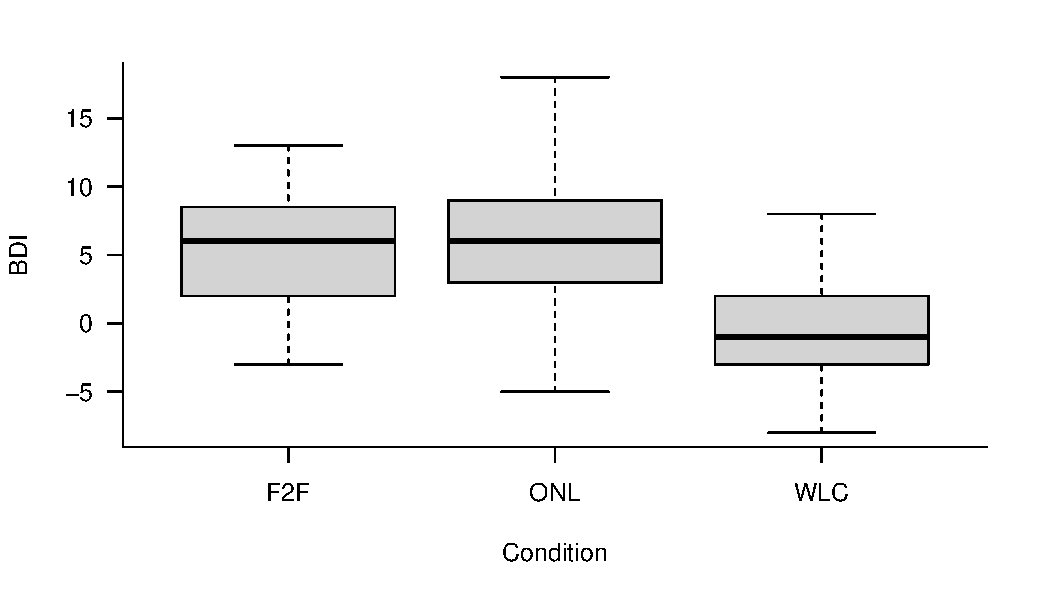
\includegraphics[width=0.95\linewidth]{10_Abbildungen/alm_10_aov_1_boxplot} \end{center}
\end{frame}

\begin{frame}[fragile]{Anwendungsszenario}
\protect\hypertarget{anwendungsszenario-4}{}
\textcolor{darkblue}{Balkendiagramm} \vspace{1mm} \tiny \setstretch{.8}

\begin{Shaded}
\begin{Highlighting}[]
\CommentTok{\# Datenselektion}
\NormalTok{fname       }\OtherTok{=} \FunctionTok{file.path}\NormalTok{(}\FunctionTok{getwd}\NormalTok{(), }\StringTok{"10\_Daten"}\NormalTok{, }\StringTok{"10\_Einfaktorielle\_Varianzanalyse\_Daten.csv"}\NormalTok{)}
\NormalTok{D           }\OtherTok{=} \FunctionTok{read.table}\NormalTok{(fname, }\AttributeTok{sep =} \StringTok{","}\NormalTok{, }\AttributeTok{header =} \ConstantTok{TRUE}\NormalTok{)}

\CommentTok{\# Datenselektion}
\NormalTok{A           }\OtherTok{=} \FunctionTok{data.frame}\NormalTok{(                          }\CommentTok{\# neuer Dataframe}
              \AttributeTok{F2F =}\NormalTok{ D}\SpecialCharTok{$}\NormalTok{BDI[D}\SpecialCharTok{$}\NormalTok{Condition }\SpecialCharTok{==} \StringTok{"F2F"}\NormalTok{],   }\CommentTok{\# F2F BDI Daten}
              \AttributeTok{ONL =}\NormalTok{ D}\SpecialCharTok{$}\NormalTok{BDI[D}\SpecialCharTok{$}\NormalTok{Condition }\SpecialCharTok{==} \StringTok{"ONL"}\NormalTok{],   }\CommentTok{\# ONL BDI Daten}
              \AttributeTok{WLC =}\NormalTok{ D}\SpecialCharTok{$}\NormalTok{BDI[D}\SpecialCharTok{$}\NormalTok{Condition }\SpecialCharTok{==} \StringTok{"WLC"}\NormalTok{])   }\CommentTok{\# WLC BDI Daten}

\CommentTok{\# Deskriptive Statistiken}
\NormalTok{groupmeans  }\OtherTok{=} \FunctionTok{colMeans}\NormalTok{(A)                          }\CommentTok{\# Gruppenmittelwerte}
\NormalTok{groupstds   }\OtherTok{=} \FunctionTok{apply}\NormalTok{(A,}\DecValTok{2}\NormalTok{,sd)                        }\CommentTok{\# Gruppenstandardabweichungen}

\CommentTok{\# Balkendiagramm}
\FunctionTok{par}\NormalTok{(                                               }\CommentTok{\# für Details siehe ?par}
\AttributeTok{family      =} \StringTok{"sans"}\NormalTok{,                              }\CommentTok{\# Serif{-}freier Fonttyp}
\AttributeTok{pty         =} \StringTok{"m"}\NormalTok{,                                 }\CommentTok{\# Maximale Abbildungsregion}
\AttributeTok{bty         =} \StringTok{"l"}\NormalTok{,                                 }\CommentTok{\# L förmige Box}
\AttributeTok{lwd         =} \DecValTok{1}\NormalTok{,                                   }\CommentTok{\# Liniendicke}
\AttributeTok{las         =} \DecValTok{1}\NormalTok{)                                   }\CommentTok{\# Horizontale Achsenbeschriftung}
\NormalTok{x }\OtherTok{=} \FunctionTok{barplot}\NormalTok{(                                       }\CommentTok{\# Ausgabe der x{-}Ordinaten (?barplot für Details)}
\NormalTok{groupmeans,}
\AttributeTok{ylim        =} \FunctionTok{c}\NormalTok{(}\SpecialCharTok{{-}}\DecValTok{5}\NormalTok{,}\DecValTok{15}\NormalTok{),}
\AttributeTok{col         =} \StringTok{"gray90"}\NormalTok{,}
\AttributeTok{ylab        =} \StringTok{"BDI"}\NormalTok{,}
\AttributeTok{xlab        =} \StringTok{"Condition"}\NormalTok{)}
\FunctionTok{arrows}\NormalTok{(                                            }\CommentTok{\# für Details siehe ?arrows}
\AttributeTok{x0          =}\NormalTok{ x,                                   }\CommentTok{\# arrow start x{-}ordinate}
\AttributeTok{y0          =}\NormalTok{ groupmeans }\SpecialCharTok{{-}}\NormalTok{ groupstds,              }\CommentTok{\# arrow start y{-}ordinate}
\AttributeTok{x1          =}\NormalTok{ x,                                   }\CommentTok{\# arrow end   x{-}ordinate}
\AttributeTok{y1          =}\NormalTok{ groupmeans }\SpecialCharTok{+}\NormalTok{ groupstds,              }\CommentTok{\# arrow end   y{-}ordinate}
\AttributeTok{code        =} \DecValTok{3}\NormalTok{,                                   }\CommentTok{\# Pfeilspitzen beiderseits}
\AttributeTok{angle       =} \DecValTok{90}\NormalTok{,                                  }\CommentTok{\# Pfeilspitzenwinkel {-}\textgreater{} Linie}
\AttributeTok{length      =} \FloatTok{0.05}\NormalTok{)                                }\CommentTok{\# Linielänge}

\CommentTok{\# PDF Speicherung}
\FunctionTok{dev.copy2pdf}\NormalTok{(}
\AttributeTok{file        =} \FunctionTok{file.path}\NormalTok{(}\FunctionTok{getwd}\NormalTok{(), }\StringTok{"10\_Abbildungen"}\NormalTok{, }\StringTok{"alm\_10\_aov\_1\_barplot.pdf"}\NormalTok{),}
\AttributeTok{width       =} \DecValTok{7}\NormalTok{,}
\AttributeTok{height      =} \DecValTok{4}\NormalTok{)}
\end{Highlighting}
\end{Shaded}
\end{frame}

\begin{frame}{Anwendungsszenario}
\protect\hypertarget{anwendungsszenario-5}{}
\textcolor{darkblue}{Balkendiagramm} \vspace{1mm}

\center

Gruppenmittelwerte \(\pm\) Gruppenstandardabweichungen

\vspace{3mm}

\begin{center}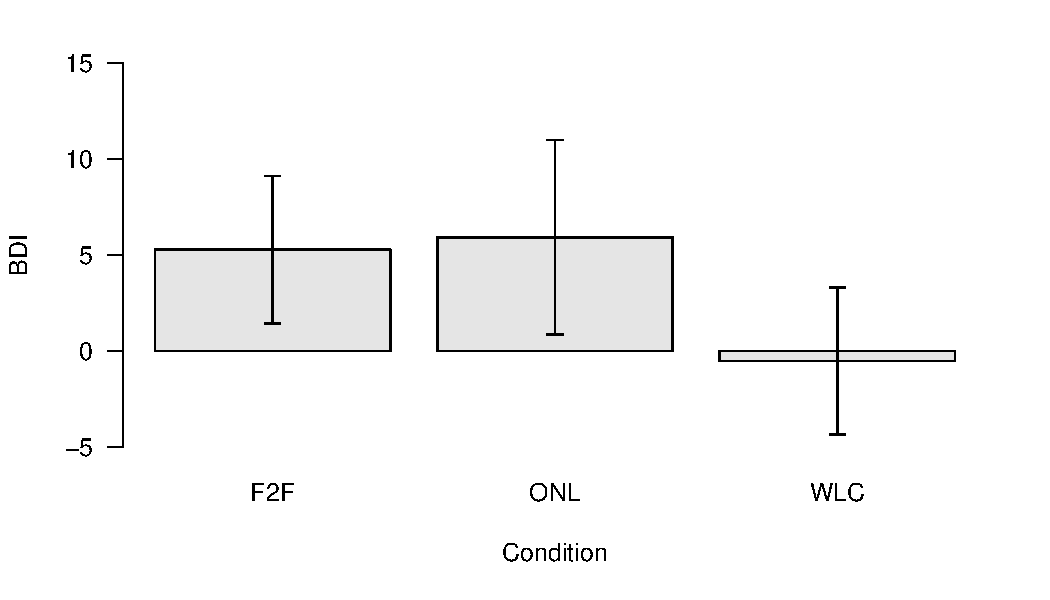
\includegraphics[width=0.95\linewidth]{10_Abbildungen/alm_10_aov_1_barplot} \end{center}
\end{frame}

\begin{frame}{}
\protect\hypertarget{section-4}{}
\large
\setstretch{2.7}
\vfill

Anwendungsszenario

\textbf{Modellformulierung}

Modellschätzung

Modellevaluation

Selbstkontrollfragen \vfill
\end{frame}

\begin{frame}{Modellformulierung}
\protect\hypertarget{modellformulierung}{}
\footnotesize
\begin{definition}[EVA Modell in Erwartungswertparameterdarstellung]
\justifying
$y_{ij}$ mit $i= 1,...,p$ und $j = 1,...,n_i$ seien Zufallsvariablen, die
die Datenpunkte eines EVA Szenarios modellieren. Dann hat das
\textit{EVA Modell in Erwartungswertparameterdarstellung} die strukturelle Form
\begin{equation}
y_{ij} = \mu_i + \varepsilon_{ij}
\mbox{ mit } \varepsilon_{ij} \sim N(0,\sigma^2)
\mbox{ u.i.v. für } i = 1,...,p, j = 1,...,n_i \mbox{ mit } \mu_i \in \mathbb{R}, \sigma^2 > 0.
\end{equation}
und die Datenverteilungsform
\begin{equation}\label{eq:aov_1_klassisch}
y_{ij} \sim N(\mu_i,\sigma^2) \mbox{ u.i.v. für } i = 1,...,p, j = 1,...,n_i \mbox{ mit } \mu_i \in \mathbb{R}, \sigma^2 > 0.
\end{equation}
Wenn $n_i := m$ für alle $i = 1,...,p$ heißt das EVA Szenario \textit{balanciert}.
\end{definition}

Bemerkungen

\begin{itemize}
\tightlist
\item
  \justifying Die Äquivalenz der beiden Modellformulierungen folgt aus
  den Ergebnissen in Einheit (5) Modellformulierung
\item
  Es handelt sich um die Generalisierung des Zweistichproben-T-Test
  Modells für unabhängige Stichproben unter Annahme identischer
  Varianzparameter von \(p = 2\) auf ein beliebiges
  \(p \in \mathbb{N}\).
\item
  Bei balancierten Varianzanalyseszenarien besteht jede Datengruppe aus
  der gleichen Anzahl von Datenpunkten.
\end{itemize}
\end{frame}

\begin{frame}{Modellformulierung}
\protect\hypertarget{modellformulierung-1}{}
\textcolor{darkblue}{Motivation der Effektdarstellung}

\footnotesize

Die Erwartungswertparameterdarstellung des EVA Modells ist ein valides
ALM, das sich in dieser Form auch in der Literatur findet (z.B. Georgii
(2009), Kapitel 12.4). Im Sinne der Konsistenz mit mehrfaktoriellen
Varianzanalysemodellen bietet sich jedoch eine Reparameterisierung der
Erwartungswertparameter an. Kern dieser Reparameterisierung ist es, den
Erwartungswertparameter der \(i\)ten Gruppe als Summe eines
\emph{gruppenübergreifenden Erwartungswertparameters}
\(\mu_0 \in \mathbb{R}\) und eines \emph{gruppenspezifischen
Effektparameters} \(\alpha_i \in \mathbb{R}\) zu modellieren,
\begin{equation}\label{eq:uber}
\mu_i := \mu_0 + \alpha_i \mbox{ für } i = 1,...,p.
\end{equation} Dabei modelliert \(\alpha_i\) den Unterschied (die
Differenz) zwischen dem \(i\)ten Erwartungswertparameter \(\mu_i\) und
dem gruppenübergreifenden Erwartungswertparameter \(\mu_0\),
\begin{equation}
\alpha_i = \mu_i - \mu_0 \mbox{ für } i = 1,...,p.
\end{equation} Allerdings hat die in dieser Form vorgenommene
Reparameterisierung einen entscheidenen Nachteil: es werden \(p\)
Erwartungswertparameter \(\mu_i, i = 1,...,p\) durch die \(p + 1\)
Parameter \(\mu_0\) und \(\alpha_i, i = 1,...,p\) dargestellt. Diese
Darstellung ist im Allgemeinen nicht eindeutig. Zum Beispiel können die
Erwartungswertparameter \(\mu_1 = 3, \mu_2 = 5, \mu_3 = 6\) sowohl durch
den gruppenspezifischen Erwartungswertparameter \(\mu_0 = 0\) und die
gruppenspezifischen Effektparameter
\(\alpha_1 = 3, \alpha_2 = 5, \alpha_3 = 6\) als auch durch den
gruppenspezifischen Erwartungswertparameter \(\mu_0 = 1\) und die
gruppenspezifischen Effektparameter
\(\alpha_1 = 2, \alpha_2 = 4, \alpha_3 = 5\) dargestellt werden. Man
sagt in diesem Kontext auch, dass das EVA Modell mit \eqref{eq:uber}
\emph{überparameterisiert} ist.
\end{frame}

\begin{frame}{Modellformulierung}
\protect\hypertarget{modellformulierung-2}{}
\textcolor{darkblue}{Motivation der Effektdarstellung}

\footnotesize

Datenanalytisch hat die Überparameterisierung eines
Varianzanalysemodells den Nachteil, dass aus \(p\) geschätzten
Erwartungswertparametern \(p + 1\) Betaparameterschätzer bestimmt werden
müssten, was wie oben gesehen nicht eindeutig erfolgen kann. Um diese
Probleme in der Effektparameterdarstellung des EVA Modells zu umgehen
und diese konsistent auf mehrfaktorielle Varianzanalysemodelle zu
übertragen, bietet sich die Einführung der Nebenbedingung
\begin{equation}
\alpha_1 := 0
\end{equation} an. Es wird also ein Effektparameter von vornherein als
``gleich Null'' angenommen. Für die gruppenspezifischen
Erwartungswertparameter ergibt sich damit \begin{align}
\begin{split}
\mu_1 & := \mu_0                                        \\
\mu_i & := \mu_0 + \alpha_i \mbox{ für } i= 2,...,p  .
\end{split}
\end{align} Hierbei wird die erste Gruppe nun als \emph{Referenzgruppe}
bezeichnet und die \(\alpha_i\) modellieren die Differenz zwischen dem
Erwartungswertparameter der \(i\)ten Gruppe und dem
Erwartungswertparameter der ersten Gruppe: \begin{equation}
\alpha_i = \mu_i - \mu_0 = \mu_i - \mu_1 \mbox{ für } i = 1,...,p.
\end{equation} \(\mu_0\) ist also kein gruppenübergreifender
Erwartungswertparameter mehr, sondern identisch mit dem
Erwartungswertparameter der ersten Gruppe. Welche tatsächliche
experimentelle Gruppe dabei als ``erste Gruppe'' definiert wird, ist
unerheblich. Entscheidend ist, dass die entsprechenden
Erwartungswertparameterschätzer
\(\hat{\mu}_0\),\(\hat{\alpha}_2, ..., \hat{\alpha}_p\) korrekt als (1)
Erwartungswertparameterschätzer der Referenzgruppe (\(\hat{\mu}_0\)) und
(2) geschätzte Erwartungswertparameterdifferenz zwischen dem
Erwartungswertparameter der Referenzgruppe und der dem
Erwartungswertparameter der \(i\)ten Gruppe
(\(\hat{\alpha}_2, ..., \hat{\alpha}_p\)) verstanden werden. Wir
formalisieren das oben Gesagte in folgendem Theorem.
\end{frame}

\begin{frame}{Modellformulierung}
\protect\hypertarget{modellformulierung-3}{}
\footnotesize
\setstretch{1.3}
\begin{theorem}[EVA Modell in Effektdarstellung mit Referenzgruppe I]
\justifying
\normalfont
Gegeben sei das EVA Modell in Erwartungswertparameterdarstellung. Dann können die
Zufallsvariablen, die die Datenpunkte des EVA Szenarios modellieren, äquivalent in
der strukturellen Form
\begin{align}\label{eq:aov_1_effekt_1}
\begin{split}
y_{1j} & = \mu_0 + \varepsilon_{1j} \quad\quad\,\,  \mbox{ mit }  \varepsilon_{1j} \sim N(0,\sigma^2) \mbox{ u.i.v. für } j = 1,...,n_1              \\
y_{ij} & = \mu_0 + \alpha_i + \varepsilon_{ij}      \mbox{ mit } \varepsilon_{ij} \sim N(0,\sigma^2) \mbox{ u.i.v. für } i = 2,...,p, j = 1,...,n_i
\end{split}
\end{align}
mit
\begin{equation}
\alpha_i := \mu_i - \mu_1 \mbox{ für } i = 2,...,p
\end{equation}
und in der entsprechenden Datenverteilungsform
\begin{align}\label{eq:aov_1_effekt_2}
\begin{split}
y_{1j} & \sim N(\mu_0,\sigma^2)  \quad\quad\,\, \mbox{ u.i.v. für } j = 1,...,n_i \mbox{ mit } \mu_1 \in \mathbb{R}, \sigma^2 > 0 \\
y_{ij} & \sim N(\mu_0 + \alpha_i,\sigma^2)      \mbox{ u.i.v. für } i = 2,..., p, j = 1,...,n_i \mbox{ mit } \alpha_i \in \mathbb{R}, \sigma^2 > 0 \\
\end{split}
\end{align}
geschrieben werden. Wir nennen \eqref{eq:aov_1_effekt_1} und \eqref{eq:aov_1_effekt_2}
strukturelle und Datenverteilungsform des \textit{EVA Modells in Effektdarstellung
mit Referenzgruppe}.
\end{theorem}
\vspace{-2mm}
\footnotesize

\underline{Beweis}

Es gilt \begin{equation}
\mu_i = \mu_0 + \mu_i - \mu_0.
\end{equation} Die Parameterisierungen mit \(\mu_i\) und mit
\(\mu_0 + \mu_i - \mu_0\) sind also gleich und damit äquivalent. Dann
folgt aber auch \begin{equation}
\mu_i = \mu_0 + (\mu_i - \mu_0) =: \mu_0 + \alpha_i \mbox{ für } i = 1,...,p
\end{equation} Mit \(\alpha_1 := 0\) gilt dann \(\mu_1 = \mu_0\) und
\(\mu_i = \mu_0 + \alpha_i\) für \(i = 2,...,p\), wie im Theorem
behauptet.
\end{frame}

\begin{frame}{Modellformulierung}
\protect\hypertarget{modellformulierung-4}{}
\footnotesize
\vspace{2mm}
\setstretch{1.2}
\begin{theorem}[EVA Modell in Effektdarstellung mit Referenzgruppe II]
\justifying
\normalfont
Gegeben sei die strukturelle Form des EVA Modells in Effektdarstellung mit Referenzgruppe.
Dann hat dieses Modell die Designmatrixform
\begin{equation}
y = X\beta + \varepsilon \mbox{ mit } \varepsilon \sim N(0_n,\sigma^2 I_n), n := \sum_{i=1}^p n_i
\end{equation}
\begin{equation*}
\renewcommand{\arraystretch}{.8}
y
:=
\begin{pmatrix*}[c]
y_{11}  \\  \vdots  \\ y_{1n_1}
\\
y_{21}  \\  \vdots  \\ y_{2n_2}
\\      \\  \vdots  \\
\\
y_{p1}  \\  \vdots  \\ y_{pn_p}
\end{pmatrix*}
\in \mathbb{R}^n, \,
X :=
\begin{pmatrix}
1           &   0          &          &     0           \\
\vdots    &     \vdots &    \cdots  &   \vdots      \\
1           &   0          &            &   0             \\
1           &   1          &            &   0             \\
\vdots    &     \vdots &    \cdots  &   \vdots      \\
1           &   1        &              &   0           \\
              &                &                &                   \\
\vdots    &     \vdots &    \cdots  &   \vdots      \\
              &                &                &                   \\
1           &   0          &                &   1             \\
\vdots    &     \vdots &    \cdots  &   \vdots      \\
1           &   0        &              &   1             \\
\end{pmatrix}
\in \mathbb{R}^{n \times p},\,
\beta :=
\begin{pmatrix}
\mu_0       \\
\alpha_2    \\
\vdots      \\
\alpha_p
\end{pmatrix}
\in \mathbb{R}^{p}
\mbox{ und }
\sigma^2 > 0.
\end{equation*}
\end{theorem}
\vspace{-2mm}

\underline{Beweis}

Das Theorem ergibt sich direkt mit den Regeln der Matrixmultiplikation.
\end{frame}

\begin{frame}{Modellformulierung}
\protect\hypertarget{modellformulierung-5}{}
\small

\textcolor{darkblue}{Beispiel}

Es seien \begin{equation}
p = 4 \mbox{ und } n_i := 3 \mbox{ für } i = 1,...,p \mbox{, also } n = 12.
\end{equation} Dann gilt \begin{equation}
y = X\beta + \varepsilon \mbox{ mit } \varepsilon \sim N(0_{12},\sigma^2 I_{12})
\end{equation} mit \footnotesize \begin{equation}
y :=
\begin{pmatrix}
y_{11}  \\
y_{12}  \\
y_{13}  \\
y_{21}  \\
y_{22}  \\
y_{23}  \\
y_{31}  \\
y_{32}  \\
y_{33}  \\
y_{41}  \\
y_{42}  \\
y_{43}
\end{pmatrix},
\,
X :=
\begin{pmatrix}
1  &    0    &  0    &  0  \\
1  &  0  &  0  &  0  \\
1  &    0    &  0  &  0  \\
1  &    1    &  0  &    0  \\
1  &    1  &    0  &    0  \\
1  &    1  &    0    &  0  \\
1    &  0    &  1  &    0  \\
1  &    0  &  1  &  0  \\
1  &    0    &  1    &  0  \\
1  &    0    &  0  &    1  \\
1  &    0  &    0    &  1  \\
1  &    0    &  0  &    1  \\
\end{pmatrix}
\in \mathbb{R}^{12 \times 4},
\,
\beta :=
\begin{pmatrix}
\mu_0       \\
\alpha_2    \\
\alpha_3    \\
\alpha_4    \\
\end{pmatrix}
\in \mathbb{R}^{4}
\mbox{ und }
\sigma^2 > 0.
\end{equation}
\end{frame}

\begin{frame}[fragile]{Modellformulierung}
\protect\hypertarget{modellformulierung-6}{}
\vspace{2mm}

\textcolor{darkblue}{Beispiel} \vspace{1mm} \tiny \setstretch{1}

\begin{Shaded}
\begin{Highlighting}[]
\CommentTok{\# Modellformulierung}
\FunctionTok{library}\NormalTok{(MASS)                                             }\CommentTok{\# Multivariate Normalverteilung}
\NormalTok{m      }\OtherTok{=} \DecValTok{3}                                                \CommentTok{\# Anzahl von Datenpunkten der iten Gruppe}
\NormalTok{p      }\OtherTok{=} \DecValTok{4}                                                \CommentTok{\# Anzahl Gruppen}
\NormalTok{n      }\OtherTok{=}\NormalTok{ p}\SpecialCharTok{*}\NormalTok{m                                              }\CommentTok{\# Gesamtanzahl Datenpunkte}
\NormalTok{Xt     }\OtherTok{=} \FunctionTok{cbind}\NormalTok{(                                           }\CommentTok{\# Designmatrix}
         \FunctionTok{matrix}\NormalTok{(}\DecValTok{1}\NormalTok{,}\AttributeTok{nrow =}\NormalTok{ n, }\AttributeTok{ncol =} \DecValTok{1}\NormalTok{),}
         \FunctionTok{kronecker}\NormalTok{(}\FunctionTok{diag}\NormalTok{(p), }\FunctionTok{matrix}\NormalTok{(}\DecValTok{1}\NormalTok{,}\AttributeTok{nrow =}\NormalTok{ m,}\AttributeTok{ncol =} \DecValTok{1}\NormalTok{)))}
\NormalTok{X      }\OtherTok{=}\NormalTok{ Xt[,}\SpecialCharTok{{-}}\DecValTok{2}\NormalTok{]}
\NormalTok{I\_n    }\OtherTok{=} \FunctionTok{diag}\NormalTok{(n)                                          }\CommentTok{\# n x n Einheitsmatrix}
\NormalTok{beta   }\OtherTok{=} \FunctionTok{matrix}\NormalTok{(}\FunctionTok{c}\NormalTok{(}\DecValTok{1}\NormalTok{,}\DecValTok{2}\NormalTok{), }\AttributeTok{nrow =}\NormalTok{ p)                         }\CommentTok{\# \textbackslash{}beta = (\textbackslash{}mu\_0,\textbackslash{}alpha\_2,\textbackslash{}alpha\_3,\textbackslash{}alpha\_4)}
\NormalTok{sigsqr }\OtherTok{=} \DecValTok{14}                                               \CommentTok{\# \textbackslash{}sigma\^{}2}

\CommentTok{\# Datenrealisierung}
\NormalTok{y      }\OtherTok{=} \FunctionTok{mvrnorm}\NormalTok{(}\DecValTok{1}\NormalTok{, X }\SpecialCharTok{\%*\%}\NormalTok{ beta, sigsqr}\SpecialCharTok{*}\NormalTok{I\_n)               }\CommentTok{\# eine Realisierung eines n{-}dimensionalen ZVs}
\end{Highlighting}
\end{Shaded}

\begin{verbatim}
>       [,1] [,2] [,3] [,4]
>  [1,]    1    0    0    0
>  [2,]    1    0    0    0
>  [3,]    1    0    0    0
>  [4,]    1    1    0    0
>  [5,]    1    1    0    0
>  [6,]    1    1    0    0
>  [7,]    1    0    1    0
>  [8,]    1    0    1    0
>  [9,]    1    0    1    0
> [10,]    1    0    0    1
> [11,]    1    0    0    1
> [12,]    1    0    0    1
\end{verbatim}
\end{frame}

\begin{frame}{}
\protect\hypertarget{section-5}{}
\large
\setstretch{2.7}
\vfill

Anwendungsszenario

Modellformulierung

\textbf{Modellschätzung}

Modellevaluation

Selbstkontrollfragen \vfill
\end{frame}

\begin{frame}{Modellschätzung}
\protect\hypertarget{modellschuxe4tzung}{}
\footnotesize
\begin{theorem}[Betaparameterschätzung im EVA Modell]
\justifying
\normalfont
Gegeben sei die Designmatrixform des EVA in Effektdarstellung mit Referenzgruppe
Dann ergibt sich für den Betaparameterschätzer
\begin{equation}
\hat{\beta}
:= \begin{pmatrix} \hat{\mu}_0 \\ \hat{\alpha}_2        \\ \vdots \\ \hat{\alpha}_p \end{pmatrix}
= \begin{pmatrix} \bar{y}_1   \\ \bar{y}_2 - \bar{y}_1 \\ \vdots \\ \bar{y}_p - \bar{y}_1  \end{pmatrix}
\end{equation}
wobei
\begin{equation}
\bar{y}_i := \frac{1}{n_i}\sum_{j=1}^{n_i}y_{ij}
\end{equation}
das Stichprobenmittel der $i$ten Gruppe bezeichent.
\end{theorem}

Bemerkungen

\begin{itemize}
\tightlist
\item
  \justifying Der Erwartungswertparameter der ersten Gruppe wird durch
  das Stichprobenmittel der ersten Gruppe geschätzt; der Effektparameter
  der \(i\)ten Gruppe wird durch die Differenz des Stichprobenmittels
  der \(i\)ten und der ersten Gruppe geschätzt. Die Beziehung zwischen
  dem Varianzparameterschätzer \(\hat{\sigma}^2\) und dem Konzept der
  gepoolten Stichprobenvarianz betrachten wir an dieser Stelle nicht
  genauer.
\end{itemize}
\end{frame}

\begin{frame}{Modellschätzung}
\protect\hypertarget{modellschuxe4tzung-1}{}
\footnotesize
\vspace{2mm}

\underline{Beweis}

Wir halten zunächst fest, dass

\tiny

\begin{align*}
\begin{split}
X^T X
& =
\setcounter{MaxMatrixCols}{20}
\begin{pmatrix}
1 & \cdots & 1 & 1 & \cdots & 1 & & \cdots & & 1 & \cdots & 1   \\
0 & \cdots & 0 & 1 & \cdots & 1 & & \cdots & & 0 & \cdots & 0   \\
  & \vdots &   &   & \vdots &   & & \vdots & &   & \vdots &     \\
0 & \cdots & 0 & 0 & \cdots & 0 & & \cdots & & 1 & \cdots & 1   \\
\end{pmatrix}
\begin{pmatrix}
1         &     0           &             &     0       \\
\vdots  &   \vdots  &   \cdots  &   \vdots  \\
1       &   0           &               &   0       \\
1         &     1           &               &   0       \\
\vdots  &   \vdots  &   \cdots  &   \vdots  \\
1         &     1         &             &   0       \\
            &               &               &           \\
\vdots  &   \vdots  &   \cdots  &   \vdots  \\
            &               &               &           \\
1       &   0           &               &   1       \\
\vdots  &   \vdots  &   \cdots  &   \vdots  \\
1         &     0         &             &   1       \\
\end{pmatrix} \\
& =
\begin{pmatrix}
n       & n_2       & n_3       &   \cdots  & n_p       \\
n_2     & n_2       & 0         &   \cdots  & 0         \\
n_3     & 0         & n_3       &   \cdots  & 0         \\
\vdots  & \vdots    & \vdots    &   \ddots  & \vdots    \\
n_p     & 0         & 0         &   \cdots  & n_p       \\
\end{pmatrix}.
\end{split}
\end{align*}
\end{frame}

\begin{frame}{Modellschätzung}
\protect\hypertarget{modellschuxe4tzung-2}{}
\footnotesize

\underline{Beweis (fortgeführt)}

Die Inverse von \(X^TX\) ist \begin{equation}
\renewcommand{\arraystretch}{1.5}
(X^TX)^{-1} =
\begin{pmatrix*}[c]
   \frac{1}{n_1}
& -\frac{1}{n_1}
& \cdots
& -\frac{1}{n_1}
\\
  -\frac{1}{n_1}
& \frac{n_1+n_2}{n_1 n_2}
& \cdots
& \frac{1}{n_1}
\\
  \vdots
& \vdots
& \ddots
& \vdots
\\
 -\frac{1}{n_1}
& \frac{1}{n_1}
& \cdots
& \frac{n_1+n_p}{n_1 n_p}
\end{pmatrix*}.
\end{equation} So gilt zum Beispiel für \(p = 3\), dass \begin{equation}
X^T X
=
\begin{pmatrix}
n       & n_2   & n_3           \\
n_2     & n_2   & 0             \\
n_3     & 0         & n_3           \\
\end{pmatrix}
\mbox{ und }
\renewcommand{\arraystretch}{1.5}
(X^TX)^{-1} =
\begin{pmatrix*}[r]
   \frac{1}{n_1}
& -\frac{1}{n_1}
& -\frac{1}{n_1}
\\
  -\frac{1}{n_1}
& \frac{n_1+n_2}{n_1 n_2}
& \frac{1}{n_1}
\\
  -\frac{1}{n_1}
& \frac{1}{n_1}
& \frac{n_1+n_3}{n_1 n_3}
\end{pmatrix*}.
\end{equation}
\end{frame}

\begin{frame}{Modellschätzung}
\protect\hypertarget{modellschuxe4tzung-3}{}
\footnotesize

\underline{Beweis (fortgeführt)}

Wir halten weiterhin fest, dass \tiny \begin{align}
\begin{split}
\renewcommand{\arraystretch}{1}
X^Ty
& =
\setcounter{MaxMatrixCols}{20}
\begin{pmatrix}
1 & \cdots & 1 & 1 & \cdots & 1 & & \cdots & & 1 & \cdots & 1   \\
0 & \cdots & 0 & 1 & \cdots & 1 & & \cdots & & 0 & \cdots & 0   \\
  & \vdots &   &   & \vdots &   & & \vdots & &   & \vdots &     \\
0 & \cdots & 0 & 0 & \cdots & 0 & & \cdots & & 1 & \cdots & 1   \\
\end{pmatrix}
\begin{pmatrix*}[c]
y_{11}  \\  \vdots  \\ y_{1n_1}
\\
y_{21}  \\  \vdots  \\ y_{2n_2}
\\      \\  \vdots  \\
\\
y_{p1}  \\  \vdots  \\ y_{pn_p}
\end{pmatrix*}
\\
& =
\begin{pmatrix}
\sum_{i=1}^p \sum_{j=1}^{n_i} y_{ij}    \\
\sum_{j=1}^{n_2} y_{2j}                 \\
\vdots                                  \\
\sum_{j=1}^{n_p} y_{pj}                 \\
\end{pmatrix}.
\end{split}
\end{align}
\end{frame}

\begin{frame}{Modellschätzung}
\protect\hypertarget{modellschuxe4tzung-4}{}
\vspace{2mm}
\footnotesize

\underline{Beweis (fortgeführt)}

Es ergibt sich also \tiny \begin{equation}
\renewcommand{\arraystretch}{2}
\hat{\beta}
= (X^T X)^{-1}X^Ty
=
\begin{pmatrix*}[c]
   \frac{1}{n_1}
& -\frac{1}{n_1}
& \cdots
& -\frac{1}{n_1}
\\
  -\frac{1}{n_1}
& \frac{n_1+n_2}{n_1 n_2}
& \cdots
& \frac{1}{n_1}
\\
  \vdots
& \vdots
& \ddots
& \vdots
\\
 -\frac{1}{n_1}
& \frac{1}{n_1}
& \cdots
& \frac{n_1+n_p}{n_1 n_p}
\end{pmatrix*}
\begin{pmatrix}
\sum_{i=1}^p \sum_{j=1}^{n_i} y_{ij}    \\
\sum_{j=1}^{n_2} y_{2j}                 \\
\vdots                                  \\
\sum_{j=1}^{n_p} y_{pj}                 \\
\end{pmatrix}.
\end{equation} \footnotesize Für die erste Komponente von
\(\hat{\beta}\) ergibt sich damit \tiny \begin{align}
\begin{split}
\hat{\beta}_1
& =
\frac{1}{n_1}\sum_{i=1}^p \sum_{j=1}^{n_i} y_{ij}
- \frac{1}{n_1}\sum_{j=1}^{n_2} y_{2j}
- \cdots
- \frac{1}{n_1}\sum_{j=1}^{n_p} y_{pj}
\\
& =
\frac{1}{n_1}
\left(
\left(
  \sum_{j=1}^{n_1} y_{1j}
+ \sum_{j=1}^{n_2} y_{2j}
+ \cdots
+ \sum_{j=1}^{n_p} y_{pj}
\right)
- \sum_{j=1}^{n_2} y_{2j}
- \cdots
- \sum_{j=1}^{n_p} y_{pj}
\right)
\\
& = \frac{1}{n_1}\sum_{j=1}^{n_1} y_{1j}
\\
&
= \bar{y}_1.
\end{split}
\end{align}
\end{frame}

\begin{frame}{Modellschätzung}
\protect\hypertarget{modellschuxe4tzung-5}{}
\footnotesize
\vspace{2mm}

\underline{Beweis (fortgeführt)}

Für die zweite Komponente von \(\hat{\beta}\) und analog für alle
weiteren ergibt sich \tiny \begin{align}
\begin{split}
\hat{\beta}_2
& =
- \frac{1}{n_1}            \sum_{i=1}^p \sum_{j=1}^{n_i} y_{ij}
+ \frac{n_1 + n_2}{n_1n_2} \sum_{j=1}^{n_2} y_{2j}
+ \frac{1}{n_1}            \sum_{j=1}^{n_3} y_{3j}
+ \cdots
+  \frac{1}{n_1}           \sum_{j=1}^{n_p} y_{pj}
\\
& =
\frac{n_1 + n_2}{n_1n_2} \sum_{j=1}^{n_2} y_{2j}
-\frac{1}{n_1}
\left(
\left(
 \sum_{j=1}^{n_1} y_{1j}
+ \sum_{j=1}^{n_2} y_{2j}
+ \cdots
+ \sum_{j=1}^{n_p} y_{pj}
\right)
- \sum_{j=1}^{n_3} y_{3j}
- \cdots
- \sum_{j=1}^{n_p} y_{pj}
\right)
\\
& =
 \frac{n_1 + n_2}{n_1n_2} \sum_{j=1}^{n_2} y_{2j}
-\frac{1}{n_1}            \sum_{j=1}^{n_1} y_{1j}
-\frac{1}{n_1}            \sum_{j=1}^{n_2} y_{2j}
\\
& =
 \frac{n_1+n_2}{n_1n_2} \sum_{j=1}^{n_2} y_{2j}
-\frac{n_2}{n_1n_2}     \sum_{j=1}^{n_2} y_{2j}
-\frac{1}{n_1}          \sum_{j=1}^{n_1} y_{1j}
\\
& =
 \frac{n_1}{n_1n_2} \sum_{j=1}^{n_2} y_{2j}
-\frac{1}{n_1}          \sum_{j=1}^{n_1} y_{1j}
\\
& =
 \frac{1}{n_2} \sum_{j=1}^{n_2} y_{2j}
-\frac{1}{n_1} \sum_{j=1}^{n_1} y_{1j}
= \bar{y}_2 - \bar{y}_1.
\end{split}
\end{align}
\end{frame}

\begin{frame}[fragile]{Modellschätzung}
\protect\hypertarget{modellschuxe4tzung-6}{}
\tiny
\vspace{2mm}
\setstretch{.8}

\begin{Shaded}
\begin{Highlighting}[]
\CommentTok{\# Dateneinlesen}
\NormalTok{fname      }\OtherTok{=} \FunctionTok{file.path}\NormalTok{(}\FunctionTok{getwd}\NormalTok{(), }\StringTok{"10\_Daten"}\NormalTok{, }\StringTok{"10\_Einfaktorielle\_Varianzanalyse\_Daten.csv"}\NormalTok{)}
\NormalTok{D          }\OtherTok{=} \FunctionTok{read.table}\NormalTok{(fname, }\AttributeTok{sep =} \StringTok{","}\NormalTok{, }\AttributeTok{header =} \ConstantTok{TRUE}\NormalTok{)}

\CommentTok{\# Datengruppen}
\NormalTok{y\_1        }\OtherTok{=}\NormalTok{ D}\SpecialCharTok{$}\NormalTok{BDI[D}\SpecialCharTok{$}\NormalTok{Condition }\SpecialCharTok{==} \StringTok{"F2F"}\NormalTok{]                        }\CommentTok{\# BDI Differenzwerte in der F2F Gruppe}
\NormalTok{y\_2        }\OtherTok{=}\NormalTok{ D}\SpecialCharTok{$}\NormalTok{BDI[D}\SpecialCharTok{$}\NormalTok{Condition }\SpecialCharTok{==} \StringTok{"ONL"}\NormalTok{]                        }\CommentTok{\# BDI Differenzwerte in der ONL Gruppe}
\NormalTok{y\_3        }\OtherTok{=}\NormalTok{ D}\SpecialCharTok{$}\NormalTok{BDI[D}\SpecialCharTok{$}\NormalTok{Condition }\SpecialCharTok{==} \StringTok{"WLC"}\NormalTok{]                        }\CommentTok{\# BDI Differenzwerte in der ONL Gruppe}

\CommentTok{\# Modellformulierung}
\NormalTok{p          }\OtherTok{=} \DecValTok{3}                                                  \CommentTok{\# drei Gruppen}
\NormalTok{m          }\OtherTok{=} \FunctionTok{length}\NormalTok{(y\_1)                                        }\CommentTok{\# balancierters Design mit n\_i = 40}
\NormalTok{n          }\OtherTok{=}\NormalTok{ p}\SpecialCharTok{*}\NormalTok{m                                                }\CommentTok{\# Datenvektordimension}
\NormalTok{y          }\OtherTok{=} \FunctionTok{matrix}\NormalTok{(}\FunctionTok{c}\NormalTok{(y\_1, y\_2, y\_3), }\AttributeTok{nrow =}\NormalTok{ n)                 }\CommentTok{\# Datenvektor}
\NormalTok{Xt         }\OtherTok{=} \FunctionTok{cbind}\NormalTok{(                                             }\CommentTok{\# Designmatrix}
             \FunctionTok{matrix}\NormalTok{(}\DecValTok{1}\NormalTok{, }\AttributeTok{nrow =}\NormalTok{ n, }\AttributeTok{ncol =} \DecValTok{1}\NormalTok{),}
             \FunctionTok{kronecker}\NormalTok{(}\FunctionTok{diag}\NormalTok{(p), }\FunctionTok{matrix}\NormalTok{(}\DecValTok{1}\NormalTok{, }\AttributeTok{nrow =}\NormalTok{ m, }\AttributeTok{ncol =} \DecValTok{1}\NormalTok{)))}
\NormalTok{X          }\OtherTok{=}\NormalTok{ Xt[,}\SpecialCharTok{{-}}\DecValTok{2}\NormalTok{]}

\CommentTok{\# Modellschätzung}
\NormalTok{beta\_hat   }\OtherTok{=} \FunctionTok{solve}\NormalTok{(}\FunctionTok{t}\NormalTok{(X) }\SpecialCharTok{\%*\%}\NormalTok{ X) }\SpecialCharTok{\%*\%} \FunctionTok{t}\NormalTok{(X) }\SpecialCharTok{\%*\%}\NormalTok{ y                   }\CommentTok{\# Betaparameterschätzer}
\NormalTok{eps\_hat    }\OtherTok{=}\NormalTok{ y }\SpecialCharTok{{-}}\NormalTok{ X }\SpecialCharTok{\%*\%}\NormalTok{ beta\_hat                                 }\CommentTok{\# Residuenvektor}
\NormalTok{sigsqr\_hat }\OtherTok{=}\NormalTok{ (}\FunctionTok{t}\NormalTok{(eps\_hat) }\SpecialCharTok{\%*\%}\NormalTok{ eps\_hat) }\SpecialCharTok{/}\NormalTok{(n}\SpecialCharTok{{-}}\NormalTok{p)                    }\CommentTok{\# Varianzparameterschätzer}
\NormalTok{s\_sqr\_123 }\OtherTok{=}\NormalTok{ ((m}\DecValTok{{-}1}\NormalTok{)}\SpecialCharTok{*}\FunctionTok{var}\NormalTok{(y\_1) }\SpecialCharTok{+}                                   \CommentTok{\# gepoolte Stichprobenvarianz}
\NormalTok{             (m}\DecValTok{{-}1}\NormalTok{)}\SpecialCharTok{*}\FunctionTok{var}\NormalTok{(y\_2) }\SpecialCharTok{+}
\NormalTok{             (m}\DecValTok{{-}1}\NormalTok{)}\SpecialCharTok{*}\FunctionTok{var}\NormalTok{(y\_3))}\SpecialCharTok{/}\NormalTok{(m}\SpecialCharTok{+}\NormalTok{m}\SpecialCharTok{+}\NormalTok{m}\SpecialCharTok{{-}}\NormalTok{p)}

\CommentTok{\# Ausgabe}
\FunctionTok{cat}\NormalTok{(}\StringTok{"hat\{beta\}                                    : "}\NormalTok{  , beta\_hat,}
    \StringTok{"}\SpecialCharTok{\textbackslash{}n}\StringTok{bar\{y\}\_1,bar\{y\}\_2,bar\{y\}\_3                   : "}\NormalTok{, }\FunctionTok{c}\NormalTok{(}\FunctionTok{mean}\NormalTok{(y\_1),}\FunctionTok{mean}\NormalTok{(y\_2),}\FunctionTok{mean}\NormalTok{(y\_3)),}
    \StringTok{"}\SpecialCharTok{\textbackslash{}n}\StringTok{bar\{y\}\_1,bar\{y\}\_2{-}bar\{y\}\_1,bar\{y\}\_3{-}bar\{y\}\_1 : "}\NormalTok{, }\FunctionTok{c}\NormalTok{(}\FunctionTok{mean}\NormalTok{(y\_1),}\FunctionTok{mean}\NormalTok{(y\_2)}\SpecialCharTok{{-}}\FunctionTok{mean}\NormalTok{(y\_1),}\FunctionTok{mean}\NormalTok{(y\_3)}\SpecialCharTok{{-}}\FunctionTok{mean}\NormalTok{(y\_1)),}
    \StringTok{"}\SpecialCharTok{\textbackslash{}n}\StringTok{hat\{sigsqr\}                                  : "}\NormalTok{, sigsqr\_hat,}
    \StringTok{"}\SpecialCharTok{\textbackslash{}n}\StringTok{s\_123\^{}2                                      : "}\NormalTok{, s\_sqr\_123,}
    \StringTok{"}\SpecialCharTok{\textbackslash{}n}\StringTok{s\_y\^{}2                                        : "}\NormalTok{, }\FunctionTok{var}\NormalTok{(y))}
\end{Highlighting}
\end{Shaded}

\begin{verbatim}
> hat{beta}                                    :  5.28 0.65 -5.8 
> bar{y}_1,bar{y}_2,bar{y}_3                   :  5.28 5.92 -0.525 
> bar{y}_1,bar{y}_2-bar{y}_1,bar{y}_3-bar{y}_1 :  5.28 0.65 -5.8 
> hat{sigsqr}                                  :  18.4 
> s_123^2                                      :  18.4 
> s_y^2                                        :  26.6
\end{verbatim}
\end{frame}

\begin{frame}{}
\protect\hypertarget{section-6}{}
\large
\setstretch{2.7}
\vfill

Anwendungsszenario

Modellformulierung

Modellschätzung

\textbf{Modellevaluation}

Selbstkontrollfragen \vfill
\end{frame}

\begin{frame}{Modellevaluation}
\protect\hypertarget{modellevaluation}{}
\small

\textcolor{darkblue}{Vorbemerkungen und Überblick}

\footnotesize

Prinzipiell sind alle Parameterschätzwerte in einem EVA Modell von
Interesse; mit der T-Teststatistik können einzelne oder lineare
Kombinationen der Betaparameterschätzwerte im Sinne von Hypothesentests
evaluiert werden.

Nichtsdestotrotz steht im EVA Szenario häufig die Evaluation der
Nullhypothese, dass alle Effektparameter gleich Null sind im
Vordergrund. Intuitiv besagt diese Nullhypothese, dass die wahren, aber
unbekannten, Erwartungswertparameter aller Gruppen identisch sind,
formal haben wir \begin{equation}
H_0 : \alpha_i = 0 \mbox{ für alle } i = 1,...,p \Leftrightarrow \Theta_0 := \mathbb{R} \times \{0_{p-1}\}
\end{equation} und \begin{equation}
H_1 : \alpha_i \neq 0 \mbox{ für mindestens ein } i = 1,...,p \Leftrightarrow \Theta_1 := \mathbb{R}^p \setminus \mathbb{R} \times \{0_{p-1}\}
\end{equation} Zur Überprüfung von \(H_0\) wird im Allgemeinen eine
\(F\)-Teststatistik eingesetzt.

Im Folgenden entwickeln wir zunächst diese \(F\)-Teststatistik anhand
einer \emph{Quadratsummenzerlegung} der Datenvariabilität in einem EVA
Szenario und betrachten in diesem Zusammenhang auch das dem \(R^2\)
analoge Maß \(\eta^2\) der Effektstärke im EVA Szenario. Ausgestattet
mit der speziellen Form der \(F\)-Teststatistik in dem hier betrachteten
Szenario diskutieren wir dann den traditionellen EVA Hypothesentest. Wir
verzichten auf eine Analyse der Testgütefunktion und eine Diskussion der
Powerfunktion.
\end{frame}

\begin{frame}{Modellevaluation}
\protect\hypertarget{modellevaluation-1}{}
\footnotesize
\setstretch{1.2}
\begin{theorem}[Quadratsummenzerlegung bei einfaktorieller Varianzanalyse]
\justifying
\normalfont
Für $i = 1,...,p$ und $j = 1,...,n_i$ sei $y_{ij}$ die $j$te Datenvariable in der
$i$ten Gruppe eines EVA Szenarios. Weiterhin seien
\center
\vspace{1mm}
\begin{tabular}{ll}
$\bar{y} := \frac{1}{n}\sum_{i=1}^p \sum_{j=1}^{n_i} y_{ij}$         & das \textit{Gesamtstichprobenmittel}  \\\\
$\bar{y}_i =\frac{1}{n_i}\sum_{j=1}^{n_i} y_{ij}$                    & das \textit{$i$te Stichprobenmittel}  \\\\
\end{tabular}
\vspace{1mm}
\flushleft
sowie

\center
\vspace{1mm}
\begin{tabular}{ll}
$\mbox{SQT} := \sum_{i=1}^p \sum_{j=1}^{n_i} (y_{ij}-\bar{y})^{2}$   & die \textit{Total Sum of Squares}   \\\\
$\mbox{SQB} := \sum_{i=1}^p n_i(\bar{y}_i-\bar{y})^{2}$              & die \textit{Between Sum of Squares} \\\\
$\mbox{SQW} := \sum_{i=1}^p \sum_{j=1}^{n_i} (y_{ij}-\bar{y}_i)^{2}$ & die \textit{Within Sum of Squares}  \\\\
\end{tabular}
\vspace{1mm}
\flushleft
Dann gilt
\begin{equation}
\mbox{SQT} = \mbox{SQB} + \mbox{SQW}.
\end{equation}
\end{theorem}
\vspace{-2mm}

Bemerkung

\begin{itemize}
\tightlist
\item
  \justifying In Analogie zur Quadratsummenzerlegung bei einer
  Ausgleichsgerade (vgl. Einheit (3) Korrelation) wird die \emph{Within
  Sum of Squares} auch als \emph{Residual Sum of Squares} bezeichnet.
\end{itemize}
\end{frame}

\begin{frame}{Modellevaluation}
\protect\hypertarget{modellevaluation-2}{}
\footnotesize

\underline{Beweis}

Es gilt \tiny \begin{align}
\begin{split}
\mbox{SQT}
& = \sum_{i=1}^p \sum_{j=1}^{n_i}(y_{ij}-\bar{y})^{2}
\\
& = \sum_{i=1}^p \sum_{j=1}^{n_i} (y_{ij}-\bar{y}_i+\bar{y}_i-\bar{y})^2
\\
& = \sum_{i=1}^p \sum_{j=1}^{n_i} \left((y_{ij}-\bar{y}_i)+(\bar{y}_i-\bar{y}) \right)^2
\\
& = \sum_{i=1}^p \sum_{j=1}^{n_i} \left(
                                    (y_{ij}-\bar{y}_i)^2
                                  +2(y_{ij}-\bar{y}_i)(\bar{y}_i-\bar{y})
                                  +(\bar{y}_i-\bar{y})^2 \right)
\\
& = \sum_{i=1}^p \left(\sum_{j=1}^{n_i} (y_{ij}-\bar{y}_i)^2
                      +\sum_{j=1}^{n_i}  2(y_{ij}-\bar{y}_i)(\bar{y}_i-\bar{y})
                      +\sum_{j=1}^{n_i} (\bar{y}_i-\bar{y})^2 \right)
\end{split}
\end{align}
\end{frame}

\begin{frame}{Modellevaluation}
\protect\hypertarget{modellevaluation-3}{}
\footnotesize

\underline{Beweis (fortgeführt)}

und weiter \tiny \begin{align*}
\begin{split}
\mbox{SQT}
& = \sum_{i=1}^p \left(\sum_{j=1}^{n_i} (y_{ij}-\bar{y}_i)^2
                     +2(\bar{y}_i-\bar{y})\sum_{j=1}^{n_i}(y_{ij}-\bar{y}_i)
                       +n_i(\bar{y}_i-\bar{y})^2 \right)
\\
& =\sum_{i=1}^p \left(\sum_{j=1}^{n_i} (y_{ij}-\bar{y}_i)^2
                 +2(\bar{y}_i-\bar{y})\sum_{j=1}^{n_i} \left(y_{ij}-\frac{1}{n_i}\sum_{j=1}^{n_i}{y_{ij}}\right)
                 +n_i(\bar{y}_i-\bar{y})^2 \right)
\\
& =\sum_{i=1}^p \left(\sum_{j=1}^{n_i} (y_{ij}-\bar{y}_i)^2
                                       +2(\bar{y}_i-\bar{y})\left(\sum_{j=1}^{n_i} y_{ij}-\sum_{j=1}^{n_i}\left(\frac{1}{n_i}\sum_{j=1}^{n_i}{y_{ij}}\right)\right)
                                        +n_i(\bar{y}_i-\bar{y})^2 \right)
\\
& =\sum_{i=1}^p \left(\sum_{j=1}^{n_i} (y_{ij}-\bar{y}_i)^2
                                       +2(\bar{y}_i-\bar{y})\left(\sum_{j=1}^{n_i} y_{ij}-\frac{n_i}{n_i}\sum_{j=1}^{n_i}{y_{ij}}\right)
                                        +n_i(\bar{y}_i-\bar{y})^2 \right)
\end{split}
\end{align*}
\end{frame}

\begin{frame}{Modellevaluation}
\protect\hypertarget{modellevaluation-4}{}
\footnotesize

\underline{Beweis (fortgeführt)}

und weiter \tiny \begin{align}
\begin{split}
\mbox{SQT}
& =\sum_{i=1}^p \left(\sum_{j=1}^{n_i} (y_{ij}-\bar{y}_i)^2
                                       +2(\bar{y}_i-\bar{y})\left(\sum_{j=1}^{n_i} y_{ij}-\sum_{j=1}^{n_i}{y_{ij}}\right)
                                        +n_i(\bar{y}_i-\bar{y})^2 \right) \\
& =\sum_{i=1}^p \left(\sum_{j=1}^{n_i} (y_{ij}-\bar{y}_i)^2 +n_i(\bar{y}_i-\bar{y})^2 \right)
\\
& =\sum_{i=1}^p \sum_{j=1}^{n_i} (y_{ij}-\bar{y}_i)^2  + \sum_{i=1}^p n_i(\bar{y}_i-\bar{y})^2
\\
& = \mbox{SQW} + \mbox{SQB}
\end{split}
\end{align} \footnotesize

und damit direkt \begin{equation}
\mbox{SQT}  = \mbox{SQB} + \mbox{SQW}.
\end{equation}
\end{frame}

\begin{frame}{Modellevaluation}
\protect\hypertarget{modellevaluation-5}{}
\footnotesize

\begin{definition}[Effektstärkenmaß $\eta^2$]
\justifying
Für ein EVA Szenario seien die Between Sum of Squares $\mbox{SQB}$ und die
Total Sum of Squares $\mbox{SQT}$ definiert wie oben. Dann ist das \textit{Effektstärkenmaß}
$\eta^2$ definiert als
\begin{equation}
\eta^2 := \frac{\mbox{SQB}}{\mbox{SQT}}
\end{equation}
\end{definition}
\vspace{-1mm}

Bemerkungen

\begin{itemize}
\tightlist
\item
  \(\eta^2\) ist analog zum Bestimmtheitsmaß \(R^2\) der Regression
  definiert.
\item
  \(\eta^2\) gibt den Anteil der Varianz zwischen den Gruppen an der
  Gesamtvarianz der Daten an.
\item
  Mit dem Theorem zur Quadratsummenzerlegung bei EVA folgt sofort
  \(0 \le \eta^2 \le 1\), da \begin{align}
  \begin{split}
  \mbox{SQB} & = 0 \Rightarrow \mbox{SQT} = \mbox{SQW und } \eta^2 = 0 \\
  \mbox{SQW} & = 0 \Rightarrow \mbox{SQT} = \mbox{SQB und } \eta^2 = 1
  \end{split}
  \end{align}
\end{itemize}
\end{frame}

\begin{frame}{Modellevaluation}
\protect\hypertarget{modellevaluation-6}{}
\footnotesize
\begin{theorem}[F-Teststatistik]
\justifying
\normalfont
Es sei
\begin{equation}
y = X\beta + \varepsilon \mbox{ mit } \varepsilon \sim N(0_n,\sigma^2I_n)
\end{equation}
die Designmatrixform der Effektdarstellung mit Referenzgruppe des EVA Modells und
im Sinne der Definition der F-Statistik (vgl. Einheit (7) Modellevaluation) sei
dieses Modell partioniert mit $p_1 := 1$ und $p_2 := p - 1$. Weiterhin seien

\center
\vspace{1mm}
\begin{tabular}{ll}
$\mbox{MSB} := \frac{\mbox{SQB}}{p-1}$        & die \textit{Mean Between Sum of Squares} \\\\
$\mbox{MSW} := \frac{\mbox{SQW}}{n-p}$        & die \textit{Mean Within  Sum of Squares} \\\\
\end{tabular}

\flushleft
respektive. Dann gilt
\begin{equation}
F = \frac{\mbox{MSB}}{\mbox{MSW}}.
\end{equation}
\end{theorem}

Bemerkungen

\begin{itemize}
\tightlist
\item
  \(p_1 := 1\) impliziert, dass das reduzierte Modell die Designmatrix
  \(X_1 := 1_n\) hat.
\item
  \(p_1 := 1\) impliziert zudem, dass das reduzierte Modell den
  Betaparameter \(\beta := \mu_0\) hat.
\item
  \(p_1 := 1\) impliziert damit auch, dass das reduzierte Modell keine
  Effektparameter hat.
\item
  Die Zahl \(p-1\) wird auch als ``Between Freiheitsgrade'' bezeichnet.
\item
  Die Zahl \(n-p\) wird auch als ``Within Freiheitsgrade'' bezeichnet.
\end{itemize}
\end{frame}

\begin{frame}{Modellevaluation}
\protect\hypertarget{modellevaluation-7}{}
\footnotesize

\underline{Beweis}

Wir halten zunächst fest, dass für den Betaparameterschätzer des
reduzierten Modells gilt, dass \begin{align}
\begin{split}
\hat{\beta}_1
= (X_1^TX_1)^{-1}X_1^Ty
= (1_n^T 1_n)^{-1}1_n^Ty
= \frac{1}{n} \sum_{i=1}^p \sum_{j = 1}^{n_i} y_{ij}
= \bar{y}.
\end{split}
\end{align} Weiterhin ergibt sich \begin{align}
\begin{split}
\hat{\varepsilon}_1^T \hat{\varepsilon}_1
= (y - X_1\hat{\beta}_1)^T(y - X_1\hat{\beta}_1)
= (y - 1_n\bar{y})^T(y - 1_n\bar{y})
= \sum_{i=1}^p \sum_{j=1}^{n_i} (y_{ij} - \bar{y})^2
= \mbox{SQT}.
\end{split}
\end{align}

Der Betaparameterschätzer des vollständigen Modells ergibt sich wie oben
gesehen zu \tiny \begin{equation}
\renewcommand{\arraystretch}{1.4}
\hat{\beta} =
\begin{pmatrix}
\hat{\mu}_0     \\
\hat{\alpha}_2  \\
\vdots          \\
\hat{\alpha}_m
\end{pmatrix}
=
\begin{pmatrix}
 \frac{1}{n_1}\sum_{j=1}^{n_1} y_{1j}   \\
 \frac{1}{n_2}\sum_{j=1}^{n_2} y_{2j}
-\frac{1}{n_1}\sum_{j=1}^{n_1} y_{1j}   \\
\vdots \\
 \frac{1}{n_m}\sum_{j=1}^{n_m} y_{mj}
-\frac{1}{n_1}\sum_{j=1}^{n_1} y_{1j}   \\
\end{pmatrix}
=
\begin{pmatrix}
\bar{y}_1                               \\
\bar{y}_2 - \bar{y}_1                   \\
\vdots                                  \\
\bar{y}_p - \bar{y}_1                   \\
\end{pmatrix},
\end{equation} \footnotesize so dass
\end{frame}

\begin{frame}{Modellevaluation}
\protect\hypertarget{modellevaluation-8}{}
\footnotesize

\underline{Beweis (fortgeführt)}

\tiny

\begin{align*}
\renewcommand{\arraystretch}{.8}
\begin{split}
\hat{\varepsilon}^T\hat{\varepsilon}
= & (y - X\hat{\beta})^T(y - X\hat{\beta}) \\
= &
\left(
\begin{pmatrix}
y_{11}          \\
\vdots          \\
y_{1n_1}        \\
y_{21}          \\
\vdots          \\
y_{2n_2}        \\
                \\
\vdots          \\
                \\
y_{p1}          \\
\vdots          \\
y_{pn_p}        \\
\end{pmatrix}
-
\begin{pmatrix}
1       &   0       &           &   0       \\
\vdots  &   \vdots  &   \cdots  &   \vdots  \\
1       &   0       &           &   0       \\
1       &   1       &           &   0       \\
\vdots  &   \vdots  &   \cdots  &   \vdots  \\
1       &   1       &           &   0       \\
        &           &           &           \\
\vdots  &   \vdots  &   \cdots  &   \vdots  \\
        &           &           &           \\
1       &   0       &           &   1       \\
\vdots  &   \vdots  &   \cdots  &   \vdots  \\
1       &   0       &           &   1       \\
\end{pmatrix}
\begin{pmatrix}
\bar{y}_1                               \\
\bar{y}_2 - \bar{y}_1                   \\
\vdots                                  \\
\bar{y}_p - \bar{y}_1                   \\
\end{pmatrix}
\right)^T
(y - X\hat{\beta})
\end{split}
\end{align*}
\end{frame}

\begin{frame}{Modellevaluation}
\protect\hypertarget{modellevaluation-9}{}
\footnotesize

\underline{Beweis (fortgeführt)}

und weiter \tiny \begin{align*}
\begin{split}
\hat{\varepsilon}^T\hat{\varepsilon}
& =
\begin{pmatrix}
y_{11}   - \bar{y}_1                            \\
\vdots                                          \\
y_{1n_1} - \bar{y}_1                            \\
y_{21}   - \bar{y}_1 - \bar{y}_2 + \bar{y}_1    \\
\vdots          \\
y_{2n_2} - \bar{y}_1 - \bar{y}_2 + \bar{y}_1    \\
                \\
\vdots          \\
                \\
y_{p1}   - \bar{y}_1 - \bar{y}_p + \bar{y}_1    \\
\vdots          \\
y_{pn_p}  - \bar{y}_1 - \bar{y}_p + \bar{y}_1   \\
\end{pmatrix}^T
\begin{pmatrix}
y_{11}   - \bar{y}_1                            \\
\vdots                                          \\
y_{1n_1} - \bar{y}_1                            \\
y_{21}   - \bar{y}_1 - \bar{y}_2 + \bar{y}_1    \\
\vdots          \\
y_{2n_2} - \bar{y}_1 - \bar{y}_2 + \bar{y}_1    \\
                \\
\vdots          \\
                \\
y_{p1}   - \bar{y}_1 - \bar{y}_p + \bar{y}_1    \\
\vdots          \\
y_{pn_p}  - \bar{y}_1 - \bar{y}_p + \bar{y}_1   \\
\end{pmatrix}
=
\begin{pmatrix}
y_{11}   - \bar{y}_1    \\
\vdots                  \\
y_{1n_1} - \bar{y}_1    \\
y_{21}   - \bar{y}_2    \\
\vdots                  \\
y_{2n_2} - \bar{y}_2    \\
                        \\
\vdots                  \\
                        \\
y_{p1}   - \bar{y}_p    \\
\vdots          \\
y_{pn_p} - \bar{y}_p    \\
\end{pmatrix}^T
\begin{pmatrix}
y_{11}   - \bar{y}_1    \\
\vdots                  \\
y_{1n_1} - \bar{y}_1    \\
y_{21}   - \bar{y}_2    \\
\vdots                  \\
y_{2n_2} - \bar{y}_2    \\
                        \\
\vdots                  \\
                        \\
y_{p1}   - \bar{y}_p    \\
\vdots          \\
y_{pn_p} - \bar{y}_p    \\
\end{pmatrix}
\\
& = \sum_{i=1}^p \sum_{j = 1}^{n_i} (y_{ij} - \bar{y}_i)^2 \\
& = \mbox{SQW}.
\end{split}
\end{align*}
\end{frame}

\begin{frame}{Modellevaluation}
\protect\hypertarget{modellevaluation-10}{}
\footnotesize

\underline{Beweis (fortgeführt)}

Mit dem Theorem zur Quadratsummenzerlegung bei einfaktorieller
Varianzanalyse \begin{equation}
\mbox{SQT}  =  \mbox{SQB} +  \mbox{SQW} \Leftrightarrow \mbox{SQB} = \mbox{SQT} - \mbox{SQW}
\end{equation} folgt sofort, dass \begin{align}
\begin{split}
\mbox{SQB}
& = \mbox{SQT} - \mbox{SQW} \\
& = \hat{\varepsilon}_1^T\hat{\varepsilon}_1 - \hat{\varepsilon}^T\hat{\varepsilon}.
\end{split}
\end{align} Dann aber folgt auch direkt, dass \begin{align}
\begin{split}
\frac{\mbox{MSB}}{\mbox{MSW}}
& = \frac{\frac{\mbox{SQB}}{p-1}}
       {\frac{\mbox{SQW}}{n-p}}
\\
& = \frac{\frac{\hat{\varepsilon}_1^T\hat{\varepsilon}_1 - \hat{\varepsilon}^T\hat{\varepsilon}}{p-1}}
       {\frac{\hat{\varepsilon}^T\hat{\varepsilon}}{n-p}}
\\
& =  F
\end{split}
\end{align}
\end{frame}

\begin{frame}{Modellevaluation}
\protect\hypertarget{modellevaluation-11}{}
\footnotesize

\begin{theorem}[Effektstärkenmaß $\eta^2$ und F-Teststatistik]
\justifying
\normalfont
Für ein EVA Szenario mit $p$ Gruppen und Gesamtdatenpunktanzahl $n$ seien das 
Effektstärkenmaß $\eta^2$ und die $F$-Teststatistik wie oben definiert. Dann gilt
\begin{equation}
\eta^2 = \frac{F(p-1)}{F(p-1) + (n-p)}
\end{equation}
\end{theorem}

Bemerkungen

\begin{itemize}
\tightlist
\item
  Das Verhältnis von \(F\) und \(\eta^2\) ist Analog zum Verhältnis von
  \(T\) und Cohen's \(d\).
\item
  Die gleichzeitige Angabe von \(F\) und \(\eta^2\) ist redundant.
\end{itemize}
\end{frame}

\begin{frame}{Modellevaluation}
\protect\hypertarget{modellevaluation-12}{}
\footnotesize
\setstretch{1}

\underline{Beweis}

Wir halten zunächst fest, dass \begin{equation}
F = \frac{\mbox{SQB}}{\mbox{SQW}}\cdot \frac{n-p}{p-1} 
\Leftrightarrow 
\mbox{SQB} = \frac{p-1}{n-p}\cdot \mbox{SQW} \cdot F
\end{equation} Damit folgt dann \begin{align}
\begin{split}
\eta^2
  = \frac{\mbox{SQB}}{\mbox{SQT}}  
  = \frac{\mbox{SQB}}{\mbox{SQB}+\mbox{SQW}}  
  = \frac{\frac{p-1}{n-p}\cdot \mbox{SQW} \cdot F}{\frac{p-1}{n-p}\cdot \mbox{SQW} \cdot F +\mbox{SQW}}  
& = \frac{\frac{F(p-1)}{n-p}\cdot \mbox{SQW} }{\frac{F(p-1)}{n-p}\cdot \mbox{SQW}  +\mbox{SQW}} \\
& = \frac{\frac{F(p-1)}{n-p}\cdot \mbox{SQW} }{\left(\frac{F(p-1)}{n-p} + 1 \right)\cdot \mbox{SQW}} \\
& = \frac{\frac{F(p-1)}{n-p}}{\frac{F(p-1)}{n-p} + \frac{n-p}{n-p}} \\
& = \frac{\frac{F(p-1)}{n-p}}{\frac{F(p-1) + (n-p)}{n-p}} \\
& = \frac{F(p-1)}{F(p-1)+(n-p)}
\end{split}
\end{align}
\end{frame}

\begin{frame}{Modellevaluation}
\protect\hypertarget{modellevaluation-13}{}
\setstretch{1.8}

\textcolor{darkblue}{Gliederung (vgl. WTFI Einheiten (12) - (14))}

\begin{enumerate}
[(1)]
\item
  Statistisches Modell \checkmark
\item
  Testhypothesen \checkmark
\item
  Teststatistik \checkmark
\item
  Test
\item
  Testumfangkontrolle
\item
  p-Werte
\end{enumerate}
\end{frame}

\begin{frame}{Modellevaluation}
\protect\hypertarget{modellevaluation-14}{}
\noindent (4) Test

\footnotesize
\begin{definition}[Einfaktorielle Varianzanalyse F-Test]
\justifying
Gegeben sie das Modell der einfaktoriellen Varianzanalyse sowie die zusammengesetzten
Null- und Alternativhypothesen
\begin{equation}
H_0 : \alpha_i = 0 \mbox{ für alle } i = 1,...,p \Leftrightarrow \Theta_0 := \mathbb{R} \times \{0_{p-1}\}
\end{equation}
und
\begin{equation}
H_1 : \alpha_i \neq 0 \mbox{ für mindestens ein } i = 1,...,p \Leftrightarrow \Theta_1 := \mathbb{R}^p \setminus \mathbb{R} \times \{0_{p-1}\}
\end{equation}
respektive. Weiterhin sei die F-Teststatistik definiert durch
\begin{equation}
F = \frac{\mbox{MSB}}{\mbox{MSW}}
\end{equation}
mit der Mean Sum of Squares Between $\mbox{MSB}$ und der Mean Sum of Square Within
$\mbox{MSW}$ definiert wie oben. Dann ist der \textit{einfaktoriellen Varianzanalyse F-Test (EVA F-Test)} 
definiert als der kritische Wert-basierte Test
\begin{equation}
\phi(y) := 1_{\{F \ge k\}} :=
\begin{cases}
1 & F \ge k \\
0 & F < k
\end{cases}.
\end{equation}
\end{definition}
\end{frame}

\begin{frame}{Modellevaluation}
\protect\hypertarget{modellevaluation-15}{}
\vspace{2mm}

\noindent (5) Testumfangkontrolle

\footnotesize
\begin{theorem}[Testumfangkontrolle]
\justifying
\normalfont
$\phi$ sei der F-Test zur einfaktoriellen Varianzanalyse. Dann ist $\phi$ ein
Level-$\alpha_0$-Test mit Testumfang $\alpha_0$, wenn der kritische Wert definiert
ist durch
\begin{equation}
k_{\alpha_0} := \varphi^{-1}(1-\alpha_0;p-1, n-p),
\end{equation}
wobei $\varphi^{-1}(\cdot; p-1, n-p)$ die inverse KVF der $f$-Verteilung mit
Freiheitsgradparametern $p-1$ und $n-p$ ist.
\end{theorem}

\center

Wahl von \(k_{\alpha_0} := \varphi^{-1}(1 - \alpha_0; p-1, n-p)\) mit
\(p = 3, n =12\) \(\alpha_0 := 0.05\) und Ablehnungsbereich

\begin{center}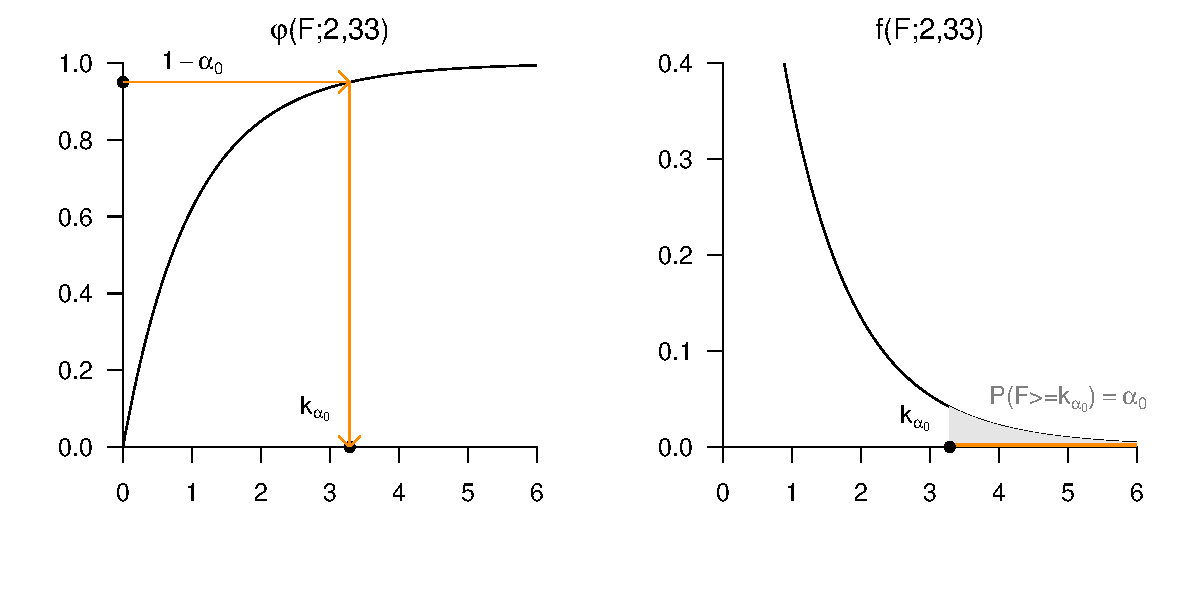
\includegraphics[width=0.7\linewidth]{10_Abbildungen/alm_10_eva_testumfang} \end{center}
\end{frame}

\begin{frame}{Modellevaluation}
\protect\hypertarget{modellevaluation-16}{}
\footnotesize

\underline{Beweis}

Die Testgütefunktion des betrachteten Tests im vorliegenden Testszenario
ist definiert als \begin{equation}
q : \mathbb{R} \to [0,1], \beta \mapsto q_\phi(\beta) := \mathbb{P}_\beta(\phi = 1).
\end{equation} Wir haben in Einheit (7) Modellevaluation gesehen, dass
die F-Teststatistik für \(p_2 = p - 1\) nach einer nichtzentralen
\(f\)-Verteilung verteilt ist, \begin{equation}
F \sim f(\delta,p-1, n-p).
\end{equation} Weiterhin ist der Ablehnungsbereich des hier betrachteten
Tests gegeben als \([k,\infty[\) Für die funktionale Form der
Testgütefunktion ergibt sich also \begin{align}
\begin{split}
\mathbb{P}_\beta(\phi = 1)
& = \mathbb{P}_\beta(F \in [k,\infty[) \\
& = \mathbb{P}_\beta(F \ge k) \\
& = 1 - \mathbb{P}_\beta(F \le k) \\
& = 1 - \varphi(k;\delta,p-1,n-p),  \\
\end{split}
\end{align} wobei \(\varphi(k;\delta,p-1,n-p)\) den Wert der KVF der
nichtzentralen \(f\)-Verteilung an der Stelle \(k\) und mit
Nichtzentralitätsparameter \(\delta\) sowie Freiheitsgradparametern
\(p-1\) und \(n-p\) bezeichnet (vgl. Einheit (7) Modellevaluation).

Damit der betrachtete Test ein Level-\(\alpha_0\)-Test ist, muss
bekanntlich gelten, dass \begin{equation}
q_\phi(\beta) \le \alpha_0 \mbox{ für alle } \beta \in \Theta_0 \mbox{ mit } \Theta_0 = \mathbb{R} \times \{0_{p-1}\}.
\end{equation}
\end{frame}

\begin{frame}{Modellevaluation}
\protect\hypertarget{modellevaluation-17}{}
\footnotesize

\underline{Beweis}

Mit der Form des Nichtzentralitätsparameters (vgl. Einheit (7)
Modellevaluation) gegeben durch \begin{equation}
\delta = \frac{1}{\sigma^2}K^T\beta\left(K^T(X^TX)^{-1}K\right)^{-1}K^T\beta
\end{equation} folgt mit \(\beta \in \Theta_0\) aus \begin{equation}
K = \begin{pmatrix} 0 \\ 1_{p-1} \end{pmatrix} \in \mathbb{R}^p \mbox{ und } \beta = \begin{pmatrix} \mu_0 \\ 0_{p-1} \end{pmatrix} \in \mathbb{R}^p 
\end{equation} dann aber \(\delta = 0\) und somit \begin{equation}
q_\phi(\beta) = 1 - \varphi(k;p-1,n-p) \mbox{ für alle } \beta \in \Theta_0.
\end{equation} wobei \(\varphi(k;p-1,n-p)\) den Wert der KVF der
\(f\)-Verteilung an der Stelle \(k\) mit Freiheitsgradparametern \(p-1\)
und \(n-p\) bezeichnet (vgl. Einheit (7) Modellevaluation). Der
Testumfang des betrachteten Tests ergibt sich nach Definition (vgl. WTFI
Einheit (12) Hypothesentests) als \begin{equation}
\alpha = \max_{{\beta \in \Theta_0}} q_{\phi}(\beta) = 1 - \varphi(k;p-1,n-p),
\end{equation} da \(q_{\phi}(\beta)\) für \(\beta \in \Theta_0\) nicht
von \(\mu_0\) abhängt. Wir müssen also lediglich zeigen, dass die Wahl
von \(k_{\alpha_0}\) wie im Theorem garantiert, dass \(\phi\) den
Testumfang \(\alpha_0\) hat. Sei also \(k := k_{\alpha_0}\). Dann gilt
für alle \(\beta \in \Theta_0\) \begin{equation}
q_\phi(\beta) 
= 1 - \varphi( \varphi^{-1}(1-\alpha_0;p-1, n-p);p-1,n-p)
= 1 - 1-\alpha_0
= \alpha_0
\end{equation} und damit ist alles gezeigt.
\end{frame}

\begin{frame}{Modellevaluation}
\protect\hypertarget{modellevaluation-18}{}
\begin{enumerate}
[(1)]
\setcounter{enumi}{6}
\tightlist
\item
  p-Wert
\end{enumerate}

\setstretch{1.2}
\footnotesize

Nach Definition ist der p-Wert das kleinste Signifikanzlevel
\(\alpha_0\), bei welchem man die Nullhypothese basierend auf einem
vorliegenden Wert der Teststatistik ablehnen würde. Wir wollen einen
vorliegenden Wert der \(F\)-Teststatistik hier mit \(f\) bezeichnen.

Bei \(F = f\) würde \(H_0\) für jedes \(\alpha_0\) mit
\(f \ge \psi^{-1}(1-\alpha_0;p-1,n-p)\) abgelehnt werden. Für ein
solches \(\alpha_0\) gilt aber \begin{equation}
\alpha_0 \ge \mathbb{P}(F \ge f),
\end{equation} denn \begin{align}
\begin{split}
f & \ge \psi^{-1}(1-\alpha_0;p-1,n-p) 
\\\Leftrightarrow
\psi(f;p-1,n-p) & \ge \psi(\psi^{-1}(1-\alpha_0;p-1,n-p), p-1,n-p) 
\\\Leftrightarrow
\psi(f;p-1,n-p) & \ge 1-\alpha_0 
\\\Leftrightarrow
\mathbb{P}(F \le f) & \ge 1-\alpha_0 
\\\Leftrightarrow
\alpha_0  & \ge 1 - \mathbb{P}(F \le f)
\\\Leftrightarrow
\alpha_0  & \ge \mathbb{P}(F \ge f)
\end{split}
\end{align} Das kleinste \(\alpha_0 \in [0,1]\) mit
\(\alpha_0 \ge \mathbb{P}(F \ge f)\) ist dann
\(\alpha_0 = \mathbb{P}(F \ge f)\), also folgt \begin{equation}
\mbox{p-Wert} = \mathbb{P}(F \ge f) = 1 - \varphi(f; p-1, n-p).
\end{equation}
\end{frame}

\begin{frame}{Modellevaluation}
\protect\hypertarget{modellevaluation-19}{}
Praktisches Vorgehen \footnotesize

\begin{itemize}
\item
  \justifying Man nimmt an, dass ein vorliegender Datensatz von \(p\)
  Gruppendatensätzen \(\upsilon_{11}, ...,\upsilon_{1n_1}\),
  \(\upsilon_{21}, ...,\upsilon_{2n_2}\), \ldots,
  \(\upsilon_{p1}, ...,\upsilon_{pn_p}\) Realisationen von
  \(y_{1j} \sim N(\mu_0,\sigma^2)\) und
  \(y_{ij} \sim N(\mu_0 + \alpha_i,\sigma^2)\) für \(i = 2,...,p\) mit
  unbekannten Parametern \(\mu_0, \alpha_i, i = 2,...,p\) und
  \(\sigma^2>0\) sind.
\item
  Man möchte entscheiden ob \(H_0 : \alpha_i = 0\) für alle
  \(i = 2,...,p\) eher zutrifft oder eher nicht.
\item
  Man wählt ein Signifikanzniveau \(\alpha_0\) und bestimmt den
  zugehörigen Freiheitsgradparameter-abhängigen kritischen Wert
  \(k_{\alpha_0}\). Zum Beispiel gilt bei Wahl von
  \(\alpha_0 := 0.05, p = 3, m = 12, i = 1,2,3\) und somit \(n = 36\),
  dass \(k_{\alpha_0} = \varphi^{-1}(1 - 0.05; 2, 33) \approx 3.28\)
  ist.
\item
  Anhand der MSB und MSW berechnet man den realisierten Wert der
  F-Teststatistik, den wir hier mit \(f\) bezeichnen.
\item
  Wenn \(f\) größer gleich \(k_{\alpha_0}\) ist, lehnt man die
  Nullhypothese ab, andernfalls nicht.
\item
  Die oben entwickelte Theorie garantiert dann, dass man im Mittel in
  höchstens \(\alpha_0 \cdot 100\) von 100 Fällen die Nullhypothese
  fälschlicherweise ablehnt.
\item
  Schließlich ergibt sich der assoziierte p-Wert der realisiertern
  F-Teststatistik \(\tilde{F}\) zu \begin{equation}
  \mbox{p-Wert} = \mathbb{P}(F \ge f) = 1 - \varphi(f; p-1, n-p)
  \end{equation}
\end{itemize}
\end{frame}

\begin{frame}[fragile]{Modellevaluation}
\protect\hypertarget{modellevaluation-20}{}
Anwendungsbeispiel

\tiny
\vspace{1mm}
\setstretch{.9}

\begin{Shaded}
\begin{Highlighting}[]
\CommentTok{\# Dateneinlesen}
\NormalTok{fname      }\OtherTok{=} \FunctionTok{file.path}\NormalTok{(}\FunctionTok{getwd}\NormalTok{(), }\StringTok{"10\_Daten"}\NormalTok{, }\StringTok{"10\_Einfaktorielle\_Varianzanalyse\_Daten.csv"}\NormalTok{)}
\NormalTok{D          }\OtherTok{=} \FunctionTok{read.table}\NormalTok{(fname, }\AttributeTok{sep =} \StringTok{","}\NormalTok{, }\AttributeTok{header =} \ConstantTok{TRUE}\NormalTok{)}

\CommentTok{\# Datengruppen}
\NormalTok{y\_1        }\OtherTok{=}\NormalTok{ D}\SpecialCharTok{$}\NormalTok{BDI[D}\SpecialCharTok{$}\NormalTok{Condition }\SpecialCharTok{==} \StringTok{"F2F"}\NormalTok{]               }\CommentTok{\# BDI Differenzwerte in der F2F Gruppe}
\NormalTok{y\_2        }\OtherTok{=}\NormalTok{ D}\SpecialCharTok{$}\NormalTok{BDI[D}\SpecialCharTok{$}\NormalTok{Condition }\SpecialCharTok{==} \StringTok{"ONL"}\NormalTok{]               }\CommentTok{\# BDI Differenzwerte in der ONL Gruppe}
\NormalTok{y\_3        }\OtherTok{=}\NormalTok{ D}\SpecialCharTok{$}\NormalTok{BDI[D}\SpecialCharTok{$}\NormalTok{Condition }\SpecialCharTok{==} \StringTok{"WLC"}\NormalTok{]               }\CommentTok{\# BDI Differenzwerte in der ONL Gruppe}

\CommentTok{\# Modellformulierung}
\NormalTok{p          }\OtherTok{=} \DecValTok{3}                                         \CommentTok{\# drei Gruppen}
\NormalTok{m          }\OtherTok{=} \FunctionTok{length}\NormalTok{(y\_1)                               }\CommentTok{\# balancierters Design mit n\_i = 40}
\NormalTok{n          }\OtherTok{=}\NormalTok{ p}\SpecialCharTok{*}\NormalTok{m                                       }\CommentTok{\# Datenvektordimension}
\NormalTok{y          }\OtherTok{=} \FunctionTok{matrix}\NormalTok{(}\FunctionTok{c}\NormalTok{(y\_1, y\_2, y\_3), }\AttributeTok{nrow =}\NormalTok{ n)        }\CommentTok{\# Datenvektor}
\NormalTok{Xt         }\OtherTok{=} \FunctionTok{cbind}\NormalTok{(                                    }\CommentTok{\# Designmatrix vollständiges Modell}
             \FunctionTok{matrix}\NormalTok{(}\DecValTok{1}\NormalTok{, }\AttributeTok{nrow =}\NormalTok{ n, }\AttributeTok{ncol =} \DecValTok{1}\NormalTok{),}
             \FunctionTok{kronecker}\NormalTok{(}\FunctionTok{diag}\NormalTok{(p),}
                       \FunctionTok{matrix}\NormalTok{(}\DecValTok{1}\NormalTok{, }\AttributeTok{nrow =}\NormalTok{ m, }\AttributeTok{ncol =} \DecValTok{1}\NormalTok{)))}
\NormalTok{X          }\OtherTok{=}\NormalTok{ Xt[,}\SpecialCharTok{{-}}\DecValTok{2}\NormalTok{]}
\NormalTok{X\_1        }\OtherTok{=}\NormalTok{ X[,}\DecValTok{1}\NormalTok{]                                     }\CommentTok{\# Designmatrix reduziertes Modell}

\CommentTok{\# F{-}Teststatistikevaluation}
\NormalTok{beta\_hat   }\OtherTok{=} \FunctionTok{solve}\NormalTok{(}\FunctionTok{t}\NormalTok{(X) }\SpecialCharTok{\%*\%}\NormalTok{ X) }\SpecialCharTok{\%*\%} \FunctionTok{t}\NormalTok{(X) }\SpecialCharTok{\%*\%}\NormalTok{ y          }\CommentTok{\# Betaparameterschätzer vollständiges Modell}
\NormalTok{beta\_hat\_1 }\OtherTok{=} \FunctionTok{solve}\NormalTok{(}\FunctionTok{t}\NormalTok{(X\_1) }\SpecialCharTok{\%*\%}\NormalTok{ X\_1) }\SpecialCharTok{\%*\%} \FunctionTok{t}\NormalTok{(X\_1) }\SpecialCharTok{\%*\%}\NormalTok{ y    }\CommentTok{\# Betaparameterschätzer reduziertes Modell}
\NormalTok{eps\_hat    }\OtherTok{=}\NormalTok{ y }\SpecialCharTok{{-}}\NormalTok{ X }\SpecialCharTok{\%*\%}\NormalTok{ beta\_hat                        }\CommentTok{\# Residuenvektor vollständiges Modell}
\NormalTok{eps\_hat\_1  }\OtherTok{=}\NormalTok{ y }\SpecialCharTok{{-}}\NormalTok{ X\_1 }\SpecialCharTok{\%*\%}\NormalTok{ beta\_hat\_1                    }\CommentTok{\# Residuenvektor reduziertes Modell}
\NormalTok{SQT        }\OtherTok{=} \FunctionTok{t}\NormalTok{(eps\_hat\_1) }\SpecialCharTok{\%*\%}\NormalTok{ eps\_hat\_1                }\CommentTok{\# Sum of Squares Total}
\NormalTok{SQW        }\OtherTok{=} \FunctionTok{t}\NormalTok{(eps\_hat)   }\SpecialCharTok{\%*\%}\NormalTok{ eps\_hat                  }\CommentTok{\# Sum of Squares Within}
\NormalTok{SQB        }\OtherTok{=}\NormalTok{ SQT }\SpecialCharTok{{-}}\NormalTok{ SQW                                 }\CommentTok{\# Sum of Squares Between}
\NormalTok{DFB        }\OtherTok{=}\NormalTok{ p }\SpecialCharTok{{-}} \DecValTok{1}                                     \CommentTok{\# Between Degrees of Freedom}
\NormalTok{DFW        }\OtherTok{=}\NormalTok{ n }\SpecialCharTok{{-}}\NormalTok{ p                                     }\CommentTok{\# Within  Degrees of Freedom}
\NormalTok{DFB        }\OtherTok{=}\NormalTok{ p }\SpecialCharTok{{-}} \DecValTok{1}                                     \CommentTok{\# Between Degrees of Freeom}
\NormalTok{MSB        }\OtherTok{=}\NormalTok{ SQB}\SpecialCharTok{/}\NormalTok{DFB                                   }\CommentTok{\# Mean Sum of Squares Between}
\NormalTok{MSW        }\OtherTok{=}\NormalTok{ SQW}\SpecialCharTok{/}\NormalTok{DFW                                   }\CommentTok{\# Mean Sum of Squares Within}
\NormalTok{Eff        }\OtherTok{=}\NormalTok{ MSB}\SpecialCharTok{/}\NormalTok{MSW                                   }\CommentTok{\# F{-}Teststatistik}
\NormalTok{p          }\OtherTok{=} \DecValTok{1} \SpecialCharTok{{-}} \FunctionTok{pf}\NormalTok{(Eff, p}\DecValTok{{-}1}\NormalTok{, n}\SpecialCharTok{{-}}\NormalTok{p)                     }\CommentTok{\# p{-}Wert}
\end{Highlighting}
\end{Shaded}
\end{frame}

\begin{frame}[fragile]{Modellevaluation}
\protect\hypertarget{modellevaluation-21}{}
Anwendungsbeispiel

\tiny
\vspace{1mm}

\begin{Shaded}
\begin{Highlighting}[]
\CommentTok{\# Ausgabe}
\FunctionTok{cat}\NormalTok{( }\StringTok{"DFB :"}\NormalTok{ , DFB,}
    \StringTok{"}\SpecialCharTok{\textbackslash{}n}\StringTok{DFW :"}\NormalTok{, DFW,}
    \StringTok{"}\SpecialCharTok{\textbackslash{}n}\StringTok{SQB :"}\NormalTok{, SQB,}
    \StringTok{"}\SpecialCharTok{\textbackslash{}n}\StringTok{SQW :"}\NormalTok{, SQW,}
    \StringTok{"}\SpecialCharTok{\textbackslash{}n}\StringTok{MSB :"}\NormalTok{, MSB,}
    \StringTok{"}\SpecialCharTok{\textbackslash{}n}\StringTok{MSW :"}\NormalTok{, MSW,}
    \StringTok{"}\SpecialCharTok{\textbackslash{}n}\StringTok{F   :"}\NormalTok{, Eff,}
    \StringTok{"}\SpecialCharTok{\textbackslash{}n}\StringTok{p   :"}\NormalTok{, }\FunctionTok{paste}\NormalTok{(p))}
\end{Highlighting}
\end{Shaded}

\begin{verbatim}
> DFB : 2 
> DFW : 117 
> SQB : 1009 
> SQW : 2153 
> MSB : 504 
> MSW : 18.4 
> F   : 27.4 
> p   : 1.7192636203589e-10
\end{verbatim}
\end{frame}

\begin{frame}[fragile]{Modellevaluation}
\protect\hypertarget{modellevaluation-22}{}
Anwendungsbeispiel

\tiny
\vspace{1mm}

\begin{Shaded}
\begin{Highlighting}[]
\CommentTok{\# Dateneinlesen}
\NormalTok{fname      }\OtherTok{=} \FunctionTok{file.path}\NormalTok{(}\FunctionTok{getwd}\NormalTok{(), }\StringTok{"10\_Daten"}\NormalTok{, }\StringTok{"10\_Einfaktorielle\_Varianzanalyse\_Daten.csv"}\NormalTok{)}
\NormalTok{D          }\OtherTok{=} \FunctionTok{read.table}\NormalTok{(fname, }\AttributeTok{sep =} \StringTok{","}\NormalTok{, }\AttributeTok{header =} \ConstantTok{TRUE}\NormalTok{)}

\CommentTok{\# Benutzung von R\textquotesingle{}s aov Funktion und Ausgabe}
\NormalTok{res.aov }\OtherTok{=} \FunctionTok{aov}\NormalTok{(D}\SpecialCharTok{$}\NormalTok{BDI }\SpecialCharTok{\textasciitilde{}}\NormalTok{ D}\SpecialCharTok{$}\NormalTok{Condition, }\AttributeTok{data =}\NormalTok{ D)}
\FunctionTok{summary}\NormalTok{(res.aov)}
\end{Highlighting}
\end{Shaded}

\begin{verbatim}
>              Df Sum Sq Mean Sq F value  Pr(>F)    
> D$Condition   2   1009     504    27.4 1.7e-10 ***
> Residuals   117   2153      18                    
> ---
> Signif. codes:  0 '***' 0.001 '**' 0.01 '*' 0.05 '.' 0.1 ' ' 1
\end{verbatim}

\vfill
\end{frame}

\begin{frame}{}
\protect\hypertarget{section-7}{}
\large
\setstretch{2.7}
\vfill

Anwendungsszenario

Modellformulierung

Modellschätzung

Modellevaluation

\textbf{Selbstkontrollfragen} \vfill
\end{frame}

\begin{frame}{Selbstkontrollfragen}
\protect\hypertarget{selbstkontrollfragen}{}
\footnotesize
\begin{enumerate}
\itemsep1mm
\item Erläutern Sie das Anwendungsszenario einer einfaktoriellen Varianzanalyse (EVA).
\item Geben Sie die Definition des EVA Modells in Erwartungswertparameterdarstellung wieder.
\item Geben Sie die strukturelle Form des EVA Modells in Effektdarstellung wieder.
\item Erläutern Sie die Motivation für die Reparameterisierung des EVA Modells
\item Welche Bedeutung haben die Parameter $\mu_0,\alpha_2,...,\alpha_p$ in der Effektparameterdarstellung des EVA Modells?
\item Warum gibt es bei $p$ Gruppen eines EVA Szenarios nur die $p-1$ Effektparameter $\alpha_2,...,\alpha_p$?
\item Geben Sie die Designmatrixform des EVA Modells in Effektdarstellung wieder.
\item Formulieren Sie die Designmatrix eines EVA Modells mit $n_i = 3$ und $p = 2$.
\item Formulieren Sie die Designmatrix eines EVA Modells mit $n_i = 2$ und $p = 5$.
\item Geben Sie das Theorem zur Betaparameterschätzung im EVA Modell wieder.
\item Mit welchen deskriptiven Statistiken werden die Parameter $\mu_0,\alpha_2,...,\alpha_p$ eines EVA Modells geschätzt? 
\item Geben Sie das Theorem zur Quadratsummenzerlegung bei einfaktorieller Varianzanalyse wieder.
\item Erläutern Sie die Begriffe Total Sum of Squares, Between Sum of Squares, Within Sum of Squares der EVA.
\item Geben Sie die Definition des Effektstärkenmaßes $\eta^2$ an.
\end{enumerate}
\end{frame}

\begin{frame}{Selbstkontrollfragen}
\protect\hypertarget{selbstkontrollfragen-1}{}
\footnotesize
\begin{enumerate}
\itemsep1mm
\setcounter{enumi}{14}
\justifying
\item Wann nimmt das Effektstärkenmaß $\eta^2$ der EVA seinen Minimalwert an und wie lautet dieser?
\item Wann nimmt das Effektstärkenmaß $\eta^2$ der EVA seinen Maximalwert an und wie lautet dieser?
\item Geben Sie das Theorem zur F-Teststatistik der EVA wieder.
\item Erläutern Sie die Begriffe Mean Between Sum of Squares und Mean Within Sum of Squares der EVA.
\item Geben Sie das Theorem zum Zusammenhang von Effektstärkenmaß $\eta^2$  und F-Teststatistik der EVA wieder.
\item Geben Sie die Definition des EVA F-Test wieder.
\item Erläutern sie die Null- und Alternativhypothesen des EVA F-Tests.
\item Geben Sie das Theorem zur Testumfangkontrolle der EVA wieder.
\item Skizzieren Sie den Beweis zur Testumfangkontrolle der EVA.
\item Geben Sie den p-Wert zum F-Test der EVA wieder.
\item Betrachten Sie die Daten zur Therapiedauer der Patient:innen in der Face-to-Face,
Online, und Waitlist Control Gruppe im Beispieldatensatz. Erstellen Sie ein Balkendiagramme 
der Gruppenmittelwerte und Gruppenstandardabweichungen und erläutern Sie dieses. 
Führen Sie zu diesen Daten einen EVA F-Test mit $\alpha := 0.05$ durch. 
Dokumentieren Sie ihre Ergebnisse. Was folgern Sie aus den sich ergebenen Resultaten?
\end{enumerate}
\end{frame}

\begin{frame}{References}
\protect\hypertarget{references}{}
\footnotesize

\hypertarget{refs}{}
\begin{CSLReferences}{1}{0}
\leavevmode\hypertarget{ref-georgii_2009}{}%
Georgii, Hans-Otto. 2009. \emph{{Stochastik: Einführung in die
Wahrscheinlichkeitstheorie und Statistik}}. 4., überarb. und erw. Aufl.
{De-Gruyter-Lehrbuch}. {Berlin}: {de Gruyter}.

\end{CSLReferences}
\end{frame}

\end{document}
